%% LyX 2.0.8.1 created this file.  For more info, see http://www.lyx.org/.
%% Do not edit unless you really know what you are doing.
\documentclass[english]{paper}
\usepackage[T1]{fontenc}
\usepackage[latin9]{inputenc}
\usepackage{color}
\usepackage{array}
\usepackage{textcomp}
\usepackage{multirow}
\usepackage{graphicx}

\makeatletter

%%%%%%%%%%%%%%%%%%%%%%%%%%%%%% LyX specific LaTeX commands.
%% Because html converters don't know tabularnewline
\providecommand{\tabularnewline}{\\}
%% A simple dot to overcome graphicx limitations
\newcommand{\lyxdot}{.}


\@ifundefined{showcaptionsetup}{}{%
 \PassOptionsToPackage{caption=false}{subfig}}
\usepackage{subfig}
\makeatother

\usepackage{babel}
\begin{document}

\section{Introduction}

Ever since Darwin's theory of evolution was proposed, cooperative
traits in animals and humans were challenging to explain. In order
to do so, Darwin's theory incorporates two novel kinds of extensions:
the genetically kinship theory that Hamilton grounded mathematically
(Hamilton,1964) and the reciprocal altruism theory (Trivers, 1971).
Both appended theories are capable to explain social altruism behavior
through natural selection. In evolutionary biology, reciprocal altruism
is a behavior whereby an organism performs a costly act that benefits
another organism with the expectation that the recipient will act
similarly later time or even in the next generation. 

The kinship theory that after landed on kin Selection and Maynar Smith
use in first time (Smith,64), talk about, on knowledge of the genetic
relationships of the organism involved, how altruistic behavior between
closely related individuals can be selected though natural selection.
This theory does not considers the altruistic act among distantly
related organisms whereas Triver's theroy does. The term \textquotedblleft{}reciprocal
altruism\textquotedblright{} was first used by Trivers to refer to
this type of behavior and therefore explain how selection favors altruistic
behaviors in the long run when there is reciprocity in the population
. Some of the most relevant and reliable examples about this type
of cooperation are the Wilkinson studies in reciprocal food sharing
behavior in vampires bats (Desmodus rotundus), (Wilkinson, 1984).
In these experiments, animals share a part of the harvested food only
to a partner that previously shared with them. Other examples, .... 

Different conditions must be fulfilled to ensure that reciprocally
altruistic behaviors will be selected. Wilkinson makes a clear summary
of these conditions : (1) the behavior must reduce a donor\textquoteright{}s
fitness relative to the selfish alternative, (2) the fitness of the
recipient must be elevated relative to a non-recipient, (3) performance
of the behavior must not depend on receipt of an immediate benefit,
(4) a mechanism for detecting individuals who receive benefits but
never pay altruistic costs has to exist, and (5) a large but indefinite
number of opportunities to exchange aid must exist within each individual\textquoteright{}s
lifetime (Wilkinson, 1987). 

Research on cooperative behaviors between non-related organisms has
gained a new impulse since Trivers connected reciprocal altruism behaviors
with the famous mathematical Prisoner's Dilemma (PD) (originally developped
by Merrill Flood and Melvin Dresher 1950). The PD game is one class
of 2x2 game that involves two players who must choose between two
options, generally called cooperation and defection. The size of the
reward delivered is established according both player's choice. If
both chose the cooperation option both get payed a certain amount
R (reward), and if both chose defection they both get payed a smaller
reward P (punishment) than R. However if one cooperates and the second
player defects, the first one gets payed S (sucker) and other receives
the best amount T (temptation) where the pay-off matrix maintains
the inequality T>R>P>S. 

Both the iterated Prisoner's Dilemma (iPD) and the Evolutionary Stable
Strategies (ESS)(von Neumann and Morgenstern, 1944; Nash, 1949) predict,
or suggest, what behavior (strategy) is likely to occur if a ESS is
adopt by the population, in such a way, no minority using a another
strategy can invade (Smith, 1974). When the 2x2 PD is played only
for one time the best ESS is Defeat strategy. Nevertheless, when the
pay-off matrix employed meets 2R>T+P and the game is played an indefinite
numbers of times, the best strategy is mutual cooperation. e.i. if
one stop reciprocity behavior the best option change to defeat. Axelrod
and Hamilton (1981) showed that some organism's symbiosis can be understood
through the reciprocal altruism's model and if organisms can remember
the outcome of at least one previous interaction and they are able
to recognize different partners, then the strategies situation includes
a much richer set of possibilities. They present a ESS for iPD that
combines robustness and stability with initial viability, called TIT
FOR TAT. This strategy arised as the winner strategy, submitted by
Anatol Rapoport, in the Robert Axelrod's computer tournament (Axelrod,
1984), because it can survive invations from other strategies. The
highly simple strategy consists in cooperating on the first move and
then doing whatever the opponent did on the preceding move. .............. 

Thus, many experimenters have tried to understand different aspects
of reciprocal altruism behavior in animals and whether non-human animals
with less cognitive abilities can solve iPD (Mendres \& Waal,2000;
Waal, 2000; Hause \& colleagues, 2003; Taborsky, 2007, 2008, 2011
and 2015, Wood, 2016; Kalenscher, 2015). Green, Price and Hamburger
(1995) assessed the iPD game on pigeons and observed that birds are
very impulsive and prefer small immediate rewards rather than big,
long-term, delayed rewards. Stephens (1995) trained blue jays (Cyanocitta
cristata) using four different pay-off matrices, where one of them
was the iPD matrix, with a special dual operant box. This study found
little cooperation in PD treatment and this findings suggest that
blue jays don't cooperate when immediate benefit is available (defect
only), even if a long-term larger benefit may exist. Then Steven and
colleages (2002 and 2005) inspired by the low levels of cooperation
observed (Gardner et al., 1984; Clements and Stephens, 1995; Flood
et al., 1983; Green et al., 1995) proposed assess over iPD frame to
the effect of a pay-off accumulation and temporal clumping treatment
to iPD game using blue jays in an apparatus that consisted of side
by side V-shaped compartments. They found that combining both accumulation
and clumping treatment birds showed a level of cooperation that scarcely
surpassed chance choice. However, Danchin and colleages (2006) criticized
the Steven's experiment arguing that each accumulation block the iPD
payoff matrix becomes stag hung matrix (whereby the temptation outcome,
T, leave to be the best reward, R>T\ensuremath{\ge}P>S) because the
bird quantify the effective amount after four trials. The Stephens'
studies is timely because it forces behavioral ecologists, and other
behavioral researcher, not only to rethink the potential importance
of temporal discounting, but also to address a number of other issues
(Mesterton-Gibbons, 2002). Indeed, we can explain from the point of
view of Operant Conditioning, the improve on cooperation levels in
Stephen's work by adding a new conditioning stimulus to the game,
transparent food storage, and in this way the game become more easy
to predict where is the maximum reward in the game. Other issue to
keep in mind is the kind of reward and punishment that is used in
the experiments, in a iPD study with rats (Viana et al., 2010) using
mimicking a tit-for-tat strategy on the opponent and positive reinforcement
and punishment in a double T-maze chamber reached a level of cooperation
that in ours further analyzed of their Markov chain diagram shown
that the strategy performed by rats was more selfish than cooperative
because it adopted an alternating decision's rule among sucker and
temptation outcomes.

.

.

Why all iPD-based studies haven't found high levels of reciprocity?
In the aforementioned previous studies, rats don't learn iPD probably
due to the fact that the test box and stimulus contingency are inadequate
for its natural expectation, i.e. the rat maybe has the ability to
achieve a approximated optimal solution but for example the length
of time used to make the contingency is longer than what rats can
keep in mind or maybe they don't realized the real difference within
outcomes in the pay-off matrix. 

Given these consideration, the present study was conduct to assess
reciprocal altruism behaviors using a particular structure that combine
iPD matrix pay-off and delay's punishment and a tit for tat opponent's
strategy. We found that this combination achieve high level of reciprocal
altruism behavior in rats.


\section{Material and Method}

All experimental procedures were approved by the ethics committee
of the IByME-CONICET and were conducted according to the NIH Guide
for Care and Use of Laboratory Animals.2.1 Subjects and Housing


\subsection{Subjects and Housing}


\subsubsection{Subject}

Two groups of male LongEvans rats (300\textendash{}330 g) of two months
of age were provided by the IBYME-CONICET. Twelves males were subjects
and six (Nstooge=6) identical rats were opponents. At weaning time
all subjects were housed in groups of two rats per cage to allow social
interaction, whereas each stooge was housed in single individual cages.
We had 12 stainless-steel cages altogether with sawdust as bedding
and metal lids. All rats were food restricted to maintain animals
at between 90-95\% or 80-85\% of free feeding body weight for subjects
and stooges respectively. All animals were kept in a well-ventilated,
temperature-controlled room (22 \textpm{} 2 \textdegree{}C) with a
12/12 h light/dark cycle (lights on at 8 am). Tap water was available
ad libitum. To ensure that animals obtained sufficient food to survive,
we provided supplementary food (at 22hs) for any rats that obtained
the average amount of pellet to maintain body weight. 

The subject was named in succesive order: 1A, 2A, 3A, 4A, 5A, 6A,
7A, 8A, 9A, 10A, 3B, 4B.


\subsubsection{Housing}

All behavioral procedures were performed during the light phase of
the light/dark cycle, using a standard operant chambers (MED associates
Inc., USA) with Med PC IV software suit (Product SOF-735) and PCI
Operating Package for up to Eight Chambers (Product MED-SYST-8) equipped
with control of multiple devices SmartCtrl (Product DIG-716B) and
pedestal mount pellet dispenser for rat, 45mg (Product ENV-203-45)
and standard operant chambers (Product ENV 008). White noise with
a flat power spectral density was used to reduce sensibility to ambient
noise. The training was perform on a single standard operant chamber
equipped with tree retractable levers and tree stimulus light over
each lever, and in the back wall placed a illuminated feeder. The
experiment was conducted in special ad hoc dual chamber. We placed
two Med association standard operant chambers facing each other in
such manner that each rat could make olfactory and eye contact through
metal windows (FIGURA 1 CAJAS). Each standard chamber was equipped
with: two not retractable levers at the sides of the same wall and
two stimulus light were placed over each levers, and in the center
put a illuminated feeder. The boxes were faced by the wall that has
levers and stimulus light. To allow the contact among rats we placed
a aluminum rectangular windows below each levers. The window's height
were such that the lever's height was 80\% of maximum height of the
forepaws while rearing (F. Cabrera et al., 2013). The subject's feeder
placed in same wall and the opponent's feeder placed in back wall.
Each feeders were equipped with a stimulus light that turn on when
foods is coming. 


\subsection{Procedures}

During the whole duration of experiment, every actor were trained
for 2 session per day for all handing, habituation, training and iPD
experiment sessions. Each typical trial began in the darkness during
5 second inter-trial interval(ITI) and then the stimulus light were
illuminated for either 45 second or until a lever was press. Before
deliver any reward the feeder light was 1 second turn on. The standard
experiment session had 30 trials. 


\subsubsection{Training procedure}


\paragraph{Handing}

At weaning time when the animals were moved to housing room started
a handing procedure to decrease the stress by experimenter manipulation
and finished when animals had 60 days old. 


\paragraph{Habituation}

The animals were habituated to the single and double operant chamber
for a days in session of 3 minute. In this treatment, there were either
no stimulus-reward contingencies or reward, only a back-light that
marked the beginning and the end of sessions.


\paragraph{Magazine}

To learn the place in which the food is given, the rat were exposed
for a days to a ``\emph{Magazine}'' procedure in the single chamber.
It consisted in variable ratio reinforcement scheduler. 


\paragraph{Shaping}

The pressing lever training on rats was done through a successive
approximations procedure, ``\emph{Shaping}'' (Mazur, 1994, page
122) on a single chamber. The chamber was equipped as described above
and was added a external lever. In this training, the external lever
was manipulated by the operator to give reward as the rat go to the
goal and finally when press lever. When the rat learned to press the
lever after light onset, the operator left to gave reward with his
lever. It training finished when the rat made the task for at least
two session. Trials procedure: each trial began when the center stimulus
light was turned on and the lever below it was ejected, then if either
inner or outer levers wasn't pressed and 45 second had elapsed, the
trials finished and not reward was given. But nevertheless, if either
inner or outer levers was pressed, the light turn-off and the feeder's
light was turned on, one second later a 45mg pellet is automatically
dispensed, when 5 second elapsed all light were turn off and the lever
was retracted, finally 5 second ITI started. The procedure was performed
during 3 days or until the rats met task goal.

Following, we exposed the rat to the same task but now the center
lever during the session never more was retracted, the lever ejected
at first trials and retracted at the last trials. In this training,
when the rat pressed lever on ITI was punished with 2 second delays
added to 5 second of ITI. This procedure went on for tree days or
until pressing rate was below one per trials.


\paragraph{Basic toggle task for subject}

The subject rats group was exposed to a training called ``toggle
8x8'' in dual iPD chamber. The purposed of the training was show
them that two lever exist and balance rat lever's preference. The
experiment was performed by 2 days in which on first day a rat use
chamber 1 and on day 2 used chamber 2. This last allow not placed
preference. The chamber communication windows were closed and any
contact was suppressed. Each rat had two lever option and two light
stimulus. When session started since the first to eighth trials only
one pair stimulus light and lever worked and the next 8 trials(9-16)
the another pair light-lever worked. What pair light lever started
was randomly and in the second day was maintained in the same way.
The trials procedure was identical to the previous one in the shaping.


\paragraph{Mimic tit for tat for opponent}

The opponent learned to develop a mimic tit for tat strategy by to
learn a basic operant task. The opponent rat group was exposed to
a fixed ratio (FR) schedule in dual operant chamber equipped in the
same way. The pair light-lever was randomly assigned in each trials
along the session. In this training, the rat must to press the lever
that had light turned on. The other lever did not work during the
trials and on the next trials the light-lever pair that worked was
pseudo-randomly assigned. Pseudo-randomly means that the assigned
was random but not allowed the same assigned for more than four time.
The training was developed during five days and the FR schedule was
increased step by step: day 1� the FR=2 and day 2� to 3� the FR=3,
then day 4� the FR=4 and finally day 5� the FR=5. If the rat press
the lever on ITI time received 2'' second delay added ITI time as
punishment. 


\subsubsection{Iterated Prisoner's Dilemma Procedure}

The main experiment was designed to study the reciprocal cooperation
lever in a iterated prisioner's dilemma game. We used a pay-off matrix
in which T>R>P>S. The T and R outcomes were positive reinforcement
and P and S was punishment. The matrix coefficient are shown in TABLE
1. Thus, If opponent choose the cooperation option (C) and the subject
choose C or defection option (D), the subject received one pellet
or 2 pellet, respectability. When the Opponent choose D and the subject
choose C or D, the subject received 8'' or 4'' delay of punishment
and no pellet in this trial. The opponent strategy was conducted by
place in which the stimulus was lighting, e.i. the opponent didn't
choose freely and the side where light was turn on, the opponent pressed
the lever. The amount pellet preference was test previously and the
rat shown more preferences for 2 pellet than 1 pellet. The delay discrimination
had been tested in \textcolor{red}{PAPER DE SELF CONTROL EN RATAS. }

\begin{table}


\caption{Prisioner's Dilemma Pay-off Matrix}


\hfill{}%
\begin{tabular}{|c|cc|}
\hline 
\multirow{2}{*}{} & \multicolumn{2}{c|}{Opponent choice}\tabularnewline
\cline{2-3} 
 & C & D\tabularnewline
\hline 
Subject choice & \multicolumn{2}{c|}{}\tabularnewline
\cline{1-1} 
\multicolumn{1}{|c||}{C} & 1 pellet & 8'' delay\tabularnewline
\multicolumn{1}{|c||}{D} & 2 pellets & 4'' delay\tabularnewline
\hline 
\end{tabular}\hfill{}

\label{table_matrixIPD}
\end{table}


In iPD experiment used a dual chamber without neither center lever
and center light. The windows cover was removed. The rats had only
two lever option and the contact between chamber was restored. There
was one chamber for the subject and one for the opponent fixed during
all the experiment, see the figure xxx(figura 1 de ARRIBA). 

The main experiment was conducted for at least 10 days and 2 session
per day. The session consisted in 30 trials. For individual subject,
the experiment was stopped, if the average behavior didn't change
along ten consecutive sessions. To some subject was exposed more than
20 days when rise its behavior tendency. 


\subsubsection{Typical\emph{ i}PD Trial Structure}

The sequence of events within a single trial was as follows. (1) The
stimulus light was turned on stating that trail was started. The focal
rats had both lights turned on (this was done throughout the iPD experiment)
and the opponent only one for the tit for tat strategy. (2) After
both rats done their response, the light was turned off and the rewards
computed. (3) The feeder's light was lighting one second before a
reward was delivered. If the opponent pressed the lever always received
one pellet irrespective the focal rat's choice. If punishment was
assigned, the focal rat feeder's light remained off and the punishment
time started, but the opponent's feed was lighted and its one pellet
reward was delivered. (5) After either five second eating time expired
or punishment time complete, all light was turned off. Then, the focal
and opponent wait the end of fixed ITI time in the darkness. The next
trials started.


\subsection{Statistical Analysis}

Al statistical analysis were performed using statistic library from
octave open source software. 


\subsubsection{Stability of cooperation}

To analysis the choice stability of rats in the iterated game, we
used the last 10 session as a pool of data due to the rat's behaviors
had reached a plateau. The mean of cooperation per rat was obtained
by count the number of times a rat chose the cooperation lever per
session over the last ten session. 


\subsubsection{Probability of cooperation after outcomes}

The animals probability to cooperate after each outcomes was assess
using a chi square test. The probability of cooperation given specific
outcomes in last trial was compared from chance, 0.5. We performed
a Chi-square goodness of fit test with bonferroni corrected value
of 0.05/n.


\subsubsection{Rate of difference outcomes}

We used Friedman's ANOVA test and multiple post-hoc pairwise comparisons
using the Nemenyi\textquoteright{}s procedure/Two-tailed tests were
performed, with the Bonferroni corrected a value of 0.0125.


\subsubsection{Markov chain diagram}

Reciprocal altruism has been widely tested by iPD, where the individual's
decision rules can be described by a transition vector t, r, p, s
that reflects the probability of cooperation when the previous trials
resulted in outcomes of R(reward), T(temptation), S(sucker) or P(punishment),
respectively (Stevens and Stephens,2004). If every component of this
vector is 0.5, the agent's decision rule is random irrespective of
the last outcome. Also we used diagram of probability of transition
between outcome to computed a complete making decision rule of each
rats.


\section{Results}


\subsection{First Phase: Iterated PD with opponent }

The experiment result are show below. To assessing whether a subject
was abled to solve the iPD game, we first need to know whether either
the subjects adopt some strategy or play in random mode. We have to
sort the type of strategy. The full data set that we record had difference
length for each rat, because after recorded 20 sessions the experiment
for each rat stop when the means of cooperation reached a plateau.
({\scriptsize{}Rat/sessions: 1A/23; 2A/33; 3A/23; 4A/23; 5A/23; 6A/31;
7A/23; 8A/50; 9A/31; 10A/29; 3B/33; 4B/23}) We compute the rat behaviors
from last ten session data set. A strategy was defined by a transition
vector that reflects the probability of cooperation when the previous
trials resulted in outcomes of R, T, S or P, respectively ($v=[p(c|t),p(c|r),p(c|p),p(c|s)]$).
The end of experiment for each rat was extended beyond 20 session
in order to the rat was progressively finding some strategy. The rat
that maintained a random strategy beyond 20 session was deserted.
When the rat maintained a not random behavior at least for ten session,
the experiment was stop. To test if rat strategy differs from chance
strategy (v={[}.5 .5 .5 .5{]}), we perform a $\chi{}^{2}$ goodness
of fit test on last ten session.

After compute the parameter $\chi{}^{2}$with bonferroni correction
for each rat we obtained two group of subject. Those who adopted some
strategy and those who did not. The figure (\ref{fig1_meansAnd significance})
shows the mean of cooperation for all rats and the asterisks marks
denoted subject that had significant difference respect the chance.
The subject 2A, 4A, 5A, 6A were removed from data pool because they
not had a fixed strategy (See Supplementary materials for the graph
of markov chain with probabilities of transition). Since the table
\ref{table_meanAndstrategies} we can see that there is a group of
8 rats with had a fixed no random strategy.

\begin{figure}
\begin{centering}
{\scriptsize{}\hfill{}}\subfloat[{\scriptsize{}Cooperation mean}]{\begin{centering}
{\scriptsize{}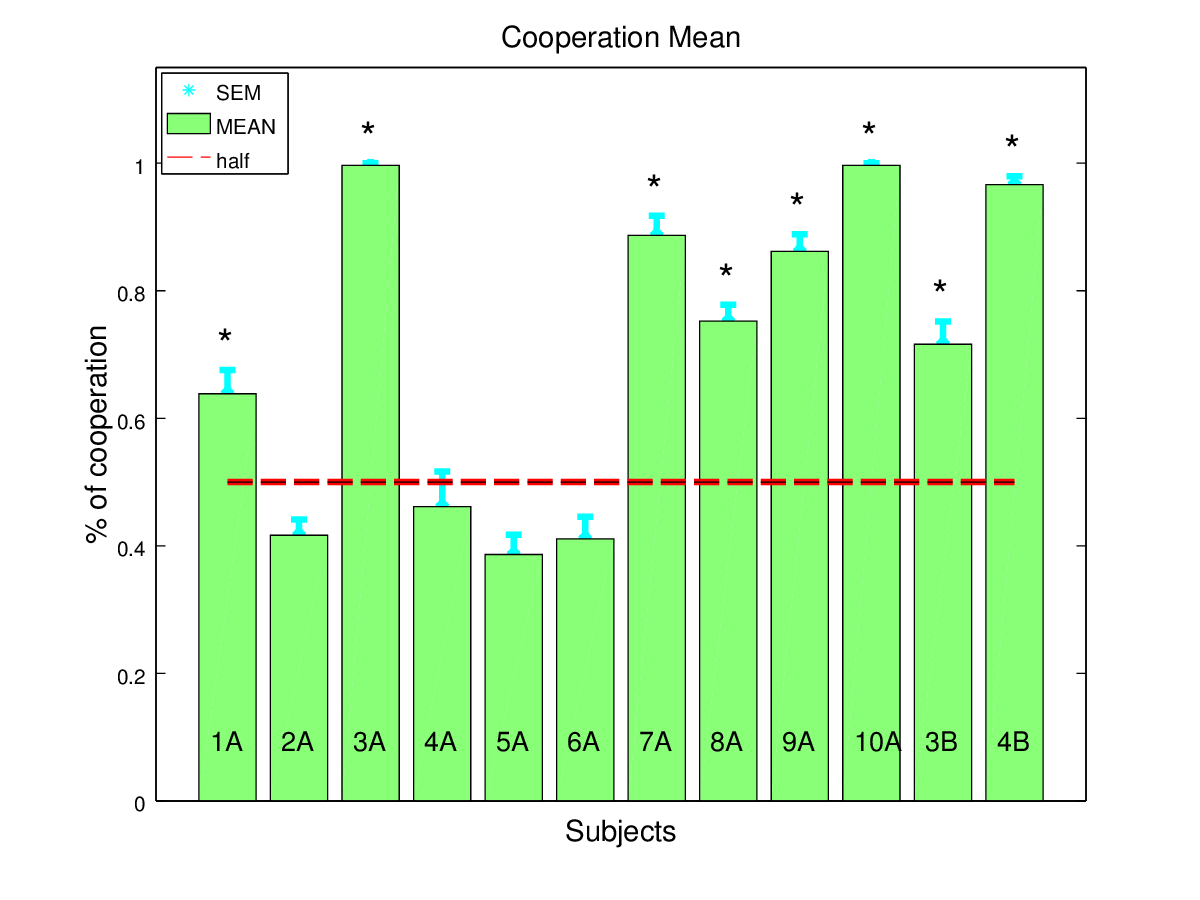
\includegraphics[width=0.45\textwidth]{/home/guille/Documents/experimento/Experimento---iPD/ExtraerDatos/figura_iPD_1_2_9s_13s/fig_finales/cooperation_mean_with_significant}}
\par\end{centering}{\scriptsize \par}

\centering{}{\scriptsize{}\label{fig1_meansAnd significance}}}{\scriptsize{}\hfill{}}\subfloat[Reward mean ]{\begin{centering}
{\scriptsize{}}
\par\end{centering}{\scriptsize \par}

\begin{centering}
{\scriptsize{}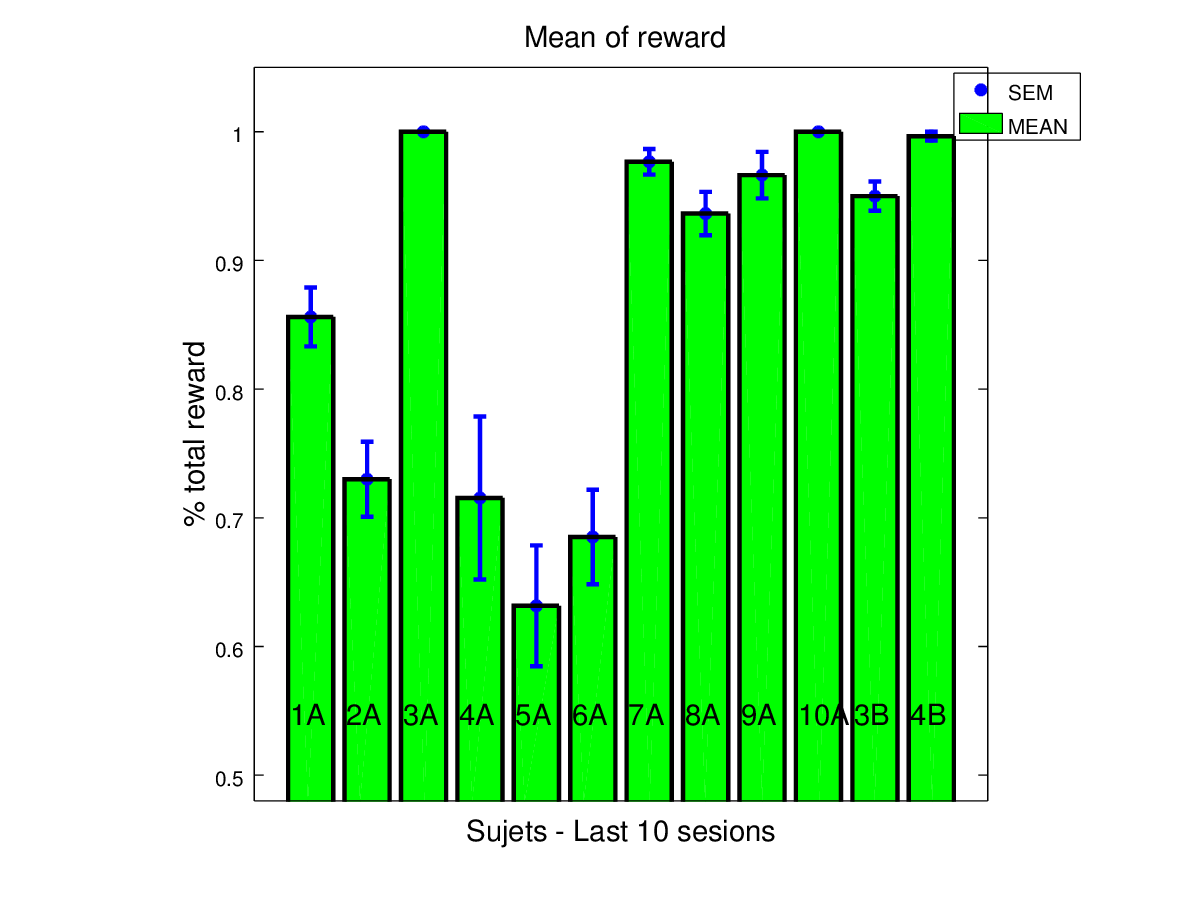
\includegraphics[width=0.45\textwidth]{/home/guille/Documents/experimento/Experimento---iPD/ExtraerDatos/figura_iPD_1_2_9s_13s/fig_finales/mean_reward}}
\par\end{centering}{\scriptsize \par}

\centering{}{\scriptsize{}\label{meanReward-1}}}{\scriptsize{}\hfill{}}
\par\end{centering}{\scriptsize \par}

{\scriptsize{}\caption{{\scriptsize{}\ref{fig1_meansAnd significance})}\textbf{\scriptsize{}Mean
and }{\scriptsize{}$\chi{}^{2}$}\textbf{\scriptsize{}test}{\scriptsize{}:
The rats with 95\% of free feeding body weight played under a matrix
pay-off T=2, R=1,P=4''delay, S=8''delay against a TFT opponent.
We show means of the numbers of times rats chose the cooperate option
($mean\pm s.e.m.$). The Asterisk denote when strategy adopted by
a rat had significant difference from chance strategy ($\chi{}^{2}$
goodness of fit test with bonferroni corrected, p>0.125). The rats
without significant difference did not surpass 0.5 probability of
cooperation. \ref{meanReward-1}) }\textbf{\scriptsize{}Means of reward.}{\scriptsize{}
Bar line shows the mean of obtained reward per session over the last
10 session ($mean\pm s.e.m.$). The rats with random strategy (not
chi-square significant) obtained the lowest level of reward, below
75\% of total reward.}}
}
\end{figure}


\begin{table}
\label{table_meanAndstrategies}\caption{{\scriptsize{}We show the mean of cooperation and the probabilities
of cooperation given each outcomes (outcomes: T, R, P and S). The
$\chi^{2}$goodness of fit with bonferroni correction was performed
used a theorical frecuency of 0.5. The significance value show the
subject that developed a specific strategy. The subject underlined
and in blue text color had significant different respect random strategy. }}


{\scriptsize{}}%
\begin{tabular}{|c|c|c|c|c|c|c|c|}
\hline 
 & {\scriptsize{}Mean} & \multicolumn{4}{c|}{Strategies} &  & \tabularnewline
\cline{1-1} \cline{3-8} 
{\scriptsize{}Subject} & {\scriptsize{}cooperation} & {\tiny{}$p(c|T)$} & {\tiny{}$p(c|R)$} & {\tiny{}$p(c|P)$} & {\tiny{}$p(c|S)$} & {\tiny{}$\chi_{bonferroni}^{2}$} & {\tiny{}$p<0.0125$}\tabularnewline
\hline 
\hline 
\textbf{\textcolor{blue}{\emph{\tiny{}1A}}} & \emph{\tiny{}$0.639$} & \emph{\tiny{}$0.525$} & \textbf{\emph{\tiny{}$0.691$}} & \emph{\tiny{}$0.644$} & \emph{\tiny{}$0.667$} & \emph{\tiny{}$17.15$} & \textcolor{blue}{\emph{\tiny{}$6.583e^{-4}$}}\tabularnewline
\hline 
\textbf{\textcolor{black}{\tiny{}2A}} & \textcolor{black}{\tiny{}$0.417$} & \textcolor{black}{\tiny{}$0.469$} & \textcolor{black}{\tiny{}$0.408$} & \textcolor{black}{\tiny{}$0.446$} & \textcolor{black}{\tiny{}$0.333$} & \textcolor{black}{\tiny{}$8.02$} & \textcolor{black}{\tiny{}$0.0456$}\tabularnewline
\hline 
\textbf{\textcolor{blue}{\tiny{}3A}} & {\tiny{}$0.997$} & {\tiny{}$1$} & \textbf{\tiny{}$0.996$} & {\tiny{}$0$} & {\tiny{}$1$} & {\tiny{}$199.30$} & \textcolor{blue}{\tiny{}$0.0000$}\tabularnewline
\hline 
\textbf{\textcolor{black}{\tiny{}4A}} & \textcolor{black}{\tiny{}$0.461$} & \textcolor{black}{\tiny{}$0.5$} & \textcolor{black}{\tiny{}$0.625$} & \textcolor{black}{\tiny{}$0.348$} & \textcolor{black}{\tiny{}$0.403$} & \textcolor{black}{\tiny{}$9.60$} & \textcolor{black}{\tiny{}$0.0223$}\tabularnewline
\hline 
\textbf{\textcolor{black}{\tiny{}5A}} & \textcolor{black}{\tiny{}$0.386$} & \textcolor{black}{\tiny{}$0.359$} & \textcolor{black}{\tiny{}$0.408$} & \textcolor{black}{\tiny{}$0.351$} & \textcolor{black}{\tiny{}$0.459$} & \textcolor{black}{\tiny{}$10.42$} & \textcolor{black}{\tiny{}$0.0152$}\tabularnewline
\hline 
\textbf{\textcolor{black}{\tiny{}6A}} & \textcolor{black}{\tiny{}$0.411$} & \textcolor{black}{\tiny{}$0.493$} & \textcolor{black}{\tiny{}$0.37$} & \textcolor{black}{\tiny{}$0.381$} & \textcolor{black}{\tiny{}$0.394$} & \textcolor{black}{\tiny{}$8.45$} & \textcolor{black}{\tiny{}$0.0375$}\tabularnewline
\hline 
\textbf{\textcolor{blue}{\tiny{}7A}} & {\tiny{}$0.886$} & {\tiny{}$0.778$} & \textbf{\tiny{}$0.904$} & {\tiny{}$0.857$} & {\tiny{}$0.885$} & {\tiny{}$103.23$} & \textcolor{blue}{\tiny{}$0.0000$}\tabularnewline
\hline 
\textbf{\textcolor{blue}{\tiny{}8A}} & {\tiny{}$0.762$} & {\tiny{}$0.638$} & \textbf{\tiny{}$0.75$} & {\tiny{}$0.682$} & {\tiny{}$0.864$} & {\tiny{}$49.38$} & \textcolor{blue}{\tiny{}$1.081e^{-10}$}\tabularnewline
\hline 
\textbf{\textcolor{blue}{\tiny{}9A}} & {\tiny{}$0.862$} & {\tiny{}$0.781$} & \textbf{\tiny{}$0.851$} & {\tiny{}$0.778$} & {\tiny{}$1$} & {\tiny{}$105.91$} & \textcolor{blue}{\tiny{}$0.0000$}\tabularnewline
\hline 
\textbf{\textcolor{blue}{\tiny{}10A}} & {\tiny{}$0.997$} & {\tiny{}$1$} & \textbf{\tiny{}$0.996$} & {\tiny{}$0$} & {\tiny{}$1$} & {\tiny{}$199.30$} & \textcolor{blue}{\tiny{}$0.0000$}\tabularnewline
\hline 
\textbf{\textcolor{blue}{\tiny{}3B}} & {\tiny{}$0.715$} & {\tiny{}$0.742$} & \textbf{\tiny{}$0.687$} & {\tiny{}$0.842$} & {\tiny{}$0.705$} & {\tiny{}$50.51$} & \textcolor{blue}{\tiny{}$6.217e^{-11}$}\tabularnewline
\hline 
\textbf{\textcolor{blue}{\tiny{}4B}} & {\tiny{}$0.966$} & {\tiny{}$0.889$} & \textbf{\tiny{}$0.97$} & {\tiny{}$1$} & {\tiny{}$1$} & {\tiny{}$174.45$} & \textcolor{blue}{\tiny{}$0.0000$}\tabularnewline
\hline 
\end{tabular}
\end{table}


In figure \ref{meanReward-1} we show the mean of reward per subject.
The rats with not random strategies got many more reward than the
removed group. But nevertheless, we show that the iPD game gives to
the random strategy group a amount that between 60\% to 70\% of total
reward.

Theoretically, when a subject play iPD against TFT opponent, its the
best strategy is All C and not TFT, because TFT against TFT when one
defeat both remain in this state and never change. Thus, if the rats
make a wrong choice, defeat, then its probability to cooperate must
be high. Analyzing the not random strategy groups behaviors, we found
that each rats had all components of strategic vector markedly above
0.5 suggesting that the rat's behaviors trend to be highly cooperative,
see table \ref{table_meanAndstrategies}. The average strategy over
all subject (blue color on table \ref{table_meanAndstrategies}) showed
that each rat has a high level of cooperation. Also we calculated
the mean and s.e.m. of cooperation choice in the groups, $0.852\pm0.0482$
and the average strategy,\textbf{ $p(c|T)=0.794$, $p(c|R)=0.856$,
$p(c|P)=0.801$, $p(c|S)=0.890$}, tested by $\chi{}^{2}$ goodness
of fit with theory frequency $0.5$, figure \ref{fig_meanC_strategy}.
In figure \ref{outcomes rate}, the rate outcomes suggest that R outcomes(i.e.
both subject and opponent chose cooperation lever option in the trial)
had very high incidence in the experiment over the last 10 sessions
into the group. We found that exist significant difference between
outcomes rate, a Friedman's ANOVA test was performed with bonferroni
correction ($\alpha=0.0125,p>3.33e-5;\chi^{2}=23.4$) and Multiple
pairwise comparison using Nemeyi's procedure point out that all outcomes
levels are different.

\begin{figure}
\hfill{}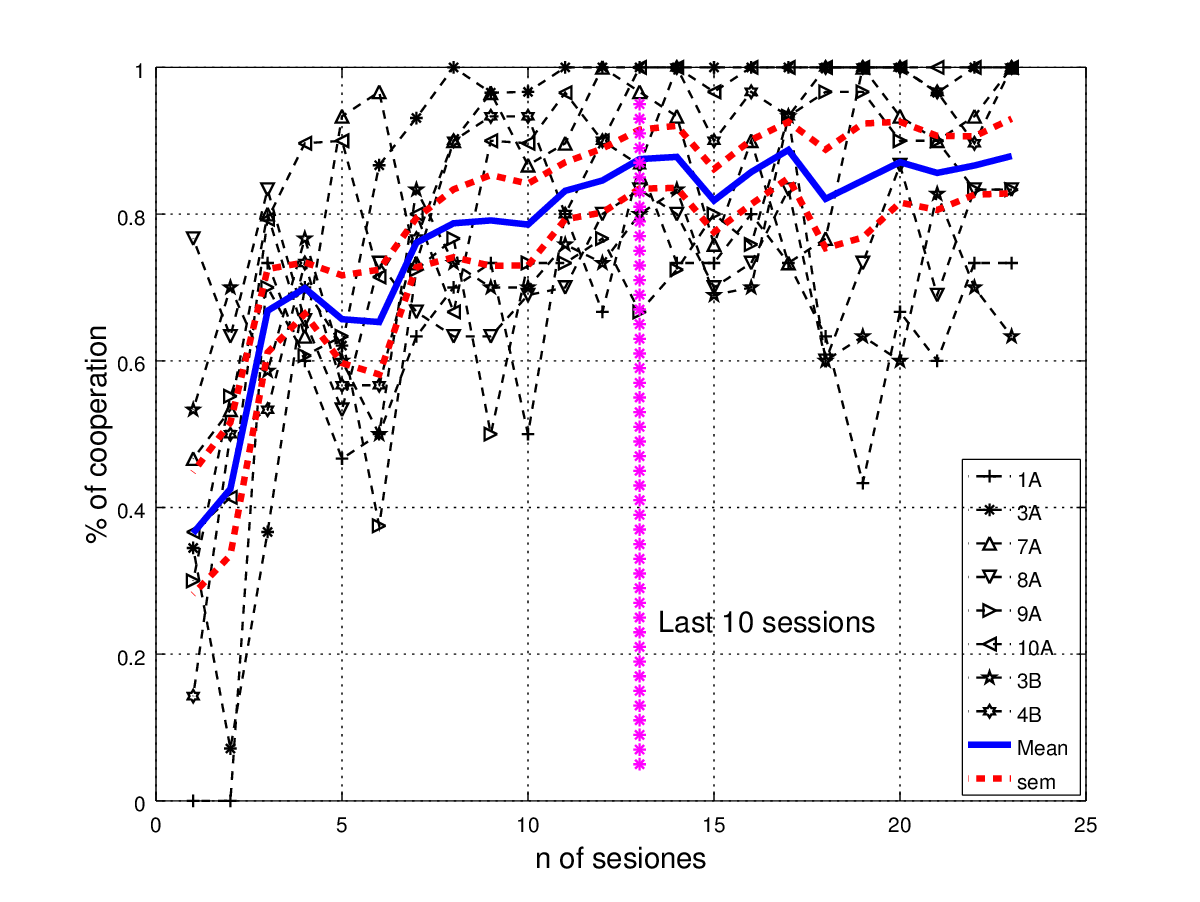
\includegraphics[width=0.6\columnwidth]{/home/guille/Documents/experimento/Experimento---iPD/ExtraerDatos/figura_iPD_1_2_9s_13s/fig_finales/cooperation_mean_sem_last23session}\hfill{}

\caption{{\scriptsize{}Evolution of cooperation choice from cooperator group
data set with the last 23 sessions. The blue and continuous and thicker
line is the means per session of the group and the dotter line is
the standard error of the mean ($mean\pm sem=0.853\pm0.0681$over
the las ten sessions). The vertical dotter line mark the pool of data
that was used to analyse the strategies adopted by the rats. }}


\label{fig_evolutionCoop}
\end{figure}


In the figure \ref{fig_evolutionCoop} we show the means of cooperation
choice per session per rats and the group means per sessions of rats
with non-random strategy. Since the number of sessions was different
along the rats, we aligned the last session of each rats and make
a pooled of data from the 23 last sessions. The means and standard
error of the means of last ten session, that represent the plateau
of the curve, was a$mean\pm sem=0.853\pm0.0681$.

\begin{figure}
\subfloat[{\scriptsize{}Mean of cooperation and means of transition vector}]{\begin{centering}
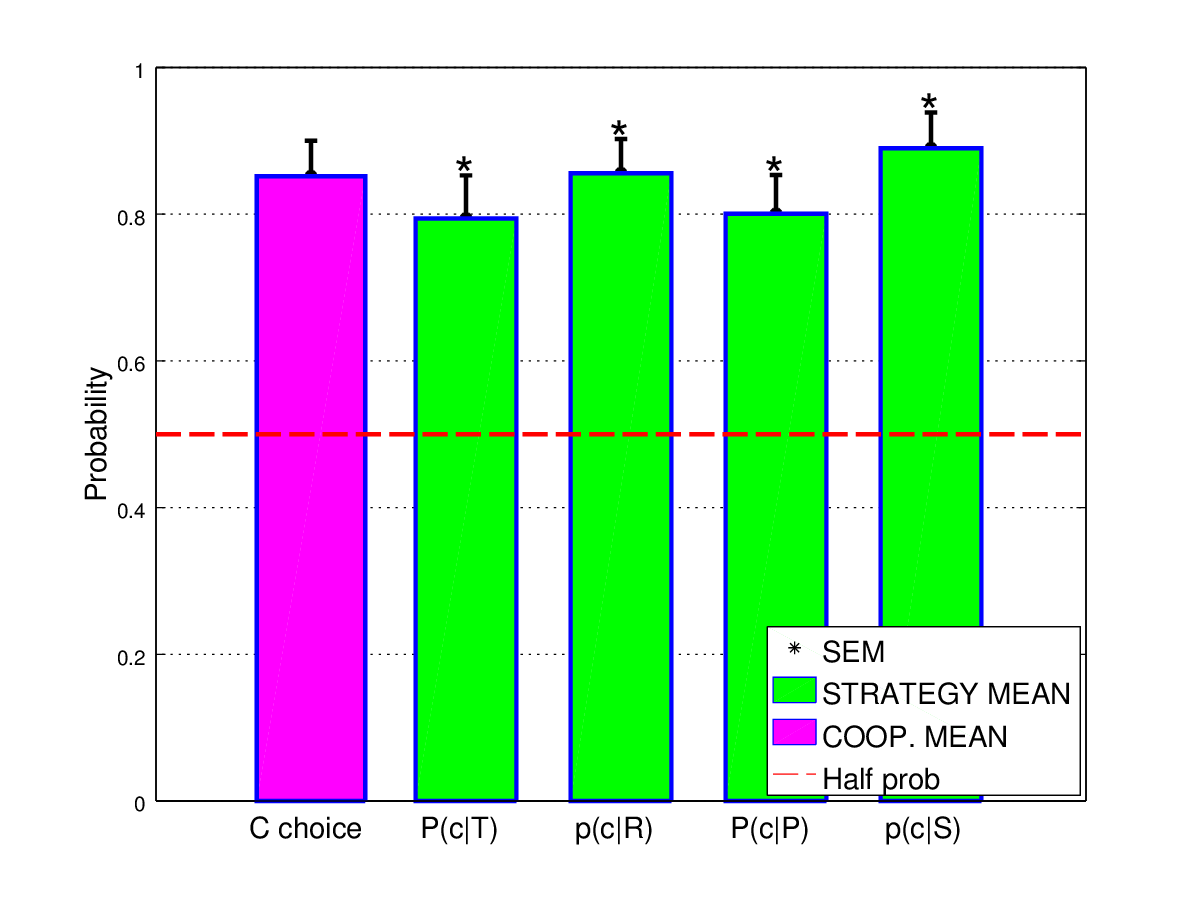
\includegraphics[width=0.45\columnwidth]{/home/guille/Documents/experimento/Experimento---iPD/ExtraerDatos/figura_iPD_1_2_9s_13s/fig_finales/mean_cooperation_and_strategy}
\par\end{centering}

\begin{centering}

\par\end{centering}

\label{fig_meanC_strategy}}\hfill{}\subfloat[{\scriptsize{}Outcomes rates over the last ten sessions.}]{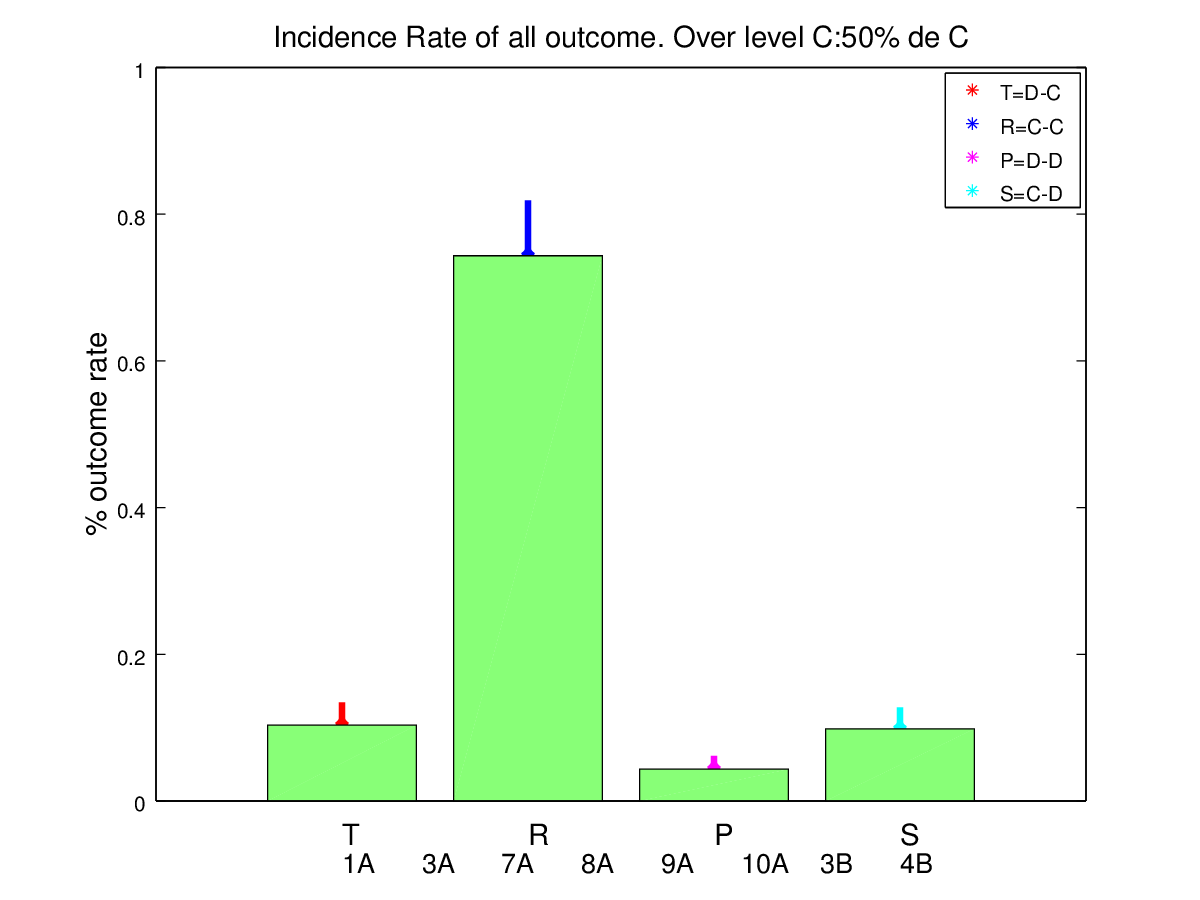
\includegraphics[width=0.45\columnwidth]{/home/guille/Documents/experimento/Experimento---iPD/ExtraerDatos/figura_iPD_1_2_9s_13s/fig_finales/outcomeRate_overLevel}



\label{outcomes rate}}

\hfill{}\subfloat[{\scriptsize{}Markov chain graph of four state}]{\begin{centering}
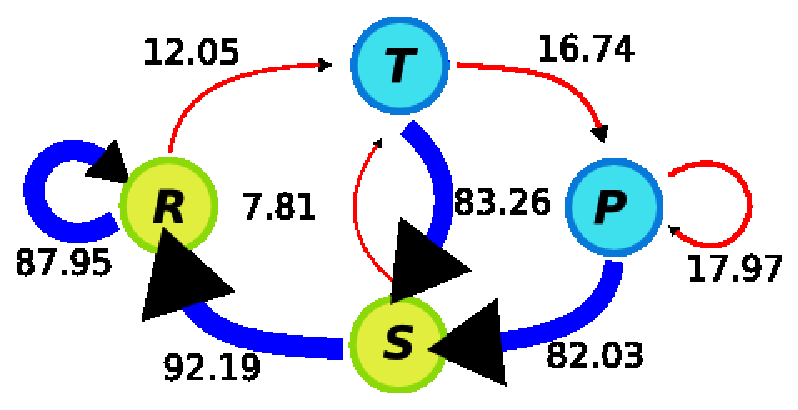
\includegraphics[width=0.4\columnwidth]{/home/guille/Documents/experimento/Experimento---iPD/ExtraerDatos/figura_iPD_1_2_9s_13s/fig_finales/g26897-6}
\par\end{centering}



\label{fig_4state_markovChain}}\hfill{}\subfloat[Markov chain graph of two state]{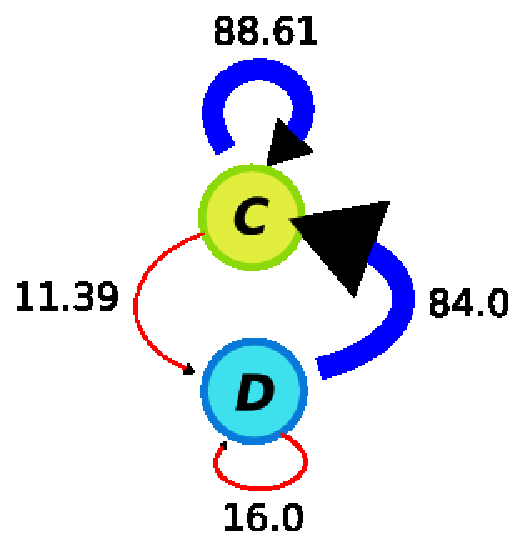
\includegraphics[width=0.3\columnwidth]{/home/guille/Documents/experimento/Experimento---iPD/ExtraerDatos/figura_iPD_1_2_9s_13s/fig_finales/g33959}



\label{fig_2state_markovChain}}\hfill{}

\caption{{\scriptsize{}\ref{fig_meanC_strategy}) Mean of cooperation over
not random strategy rats (8 rats) was performed and the measured is
shown on the first magenta bar ($mean=0.852$ and $s.e.m.=\pm0.0482$
). The next four green bars represent the mean strategy over the group
and each bar agree with the transition vector,$v=[0.794,0.856,0.801,0.890]$.
The asterisk indicates significant difference respect the half probability
of chose cooperation lever and we tested by $\chi{}^{2}$ goodness
of fit with theory frequency 0.5. \ref{outcomes rate}) The bar graph
shows the outcomes rates and suggest that R outcomes had very high
incidence in the experiment over the last 10 sessions. . We found
significant difference between outcomes (Friedman's ANOVA test was
performed with bonferroni correction ($\alpha=0.0125,p>3.3e-5;\chi^{2}=23.4$)
and Multiple pairwise comparison's using Nemeyi's procedure ). \ref{fig_4state_markovChain}
and \ref{fig_2state_markovChain}) Graph of Markov chain of four and
two state, in which the arrow represent the transition probability
between outcomes. A blue arrow signalized when the subject chose cooperate
lever given the las outcome and a red arrow signalized when it chose
defect lever. The words mean temptation (T), mutual cooperation (R),
punishment (P) and sucker (S). Pay atemption that the arrows width
are proportional to the transition probability. }}
\end{figure}


In figure \ref{fig_4state_markovChain} and \ref{fig_2state_markovChain}
we show diagrams of transition probability given the last outcomes,
respect four and two state. This diagrams means that in each trials
the subject can choose cooperation (blue arrow) or defect lever (red
arrow) with a specific probability. The arrow's width is proportional
to the probability of cooperate or to not cooperate. In both diagrams
the big blue arrow are predominates and these indicate a strong trend
to cooperate by all rats in the group. This diagrams show the rats
trend to stay on mutual cooperation or quickly come back to this state.
In all cases, the probability to cooperate was over $80\%$

\begin{figure}
\hfill{}\subfloat[Mutual Cooperation versus cooperation choice ]{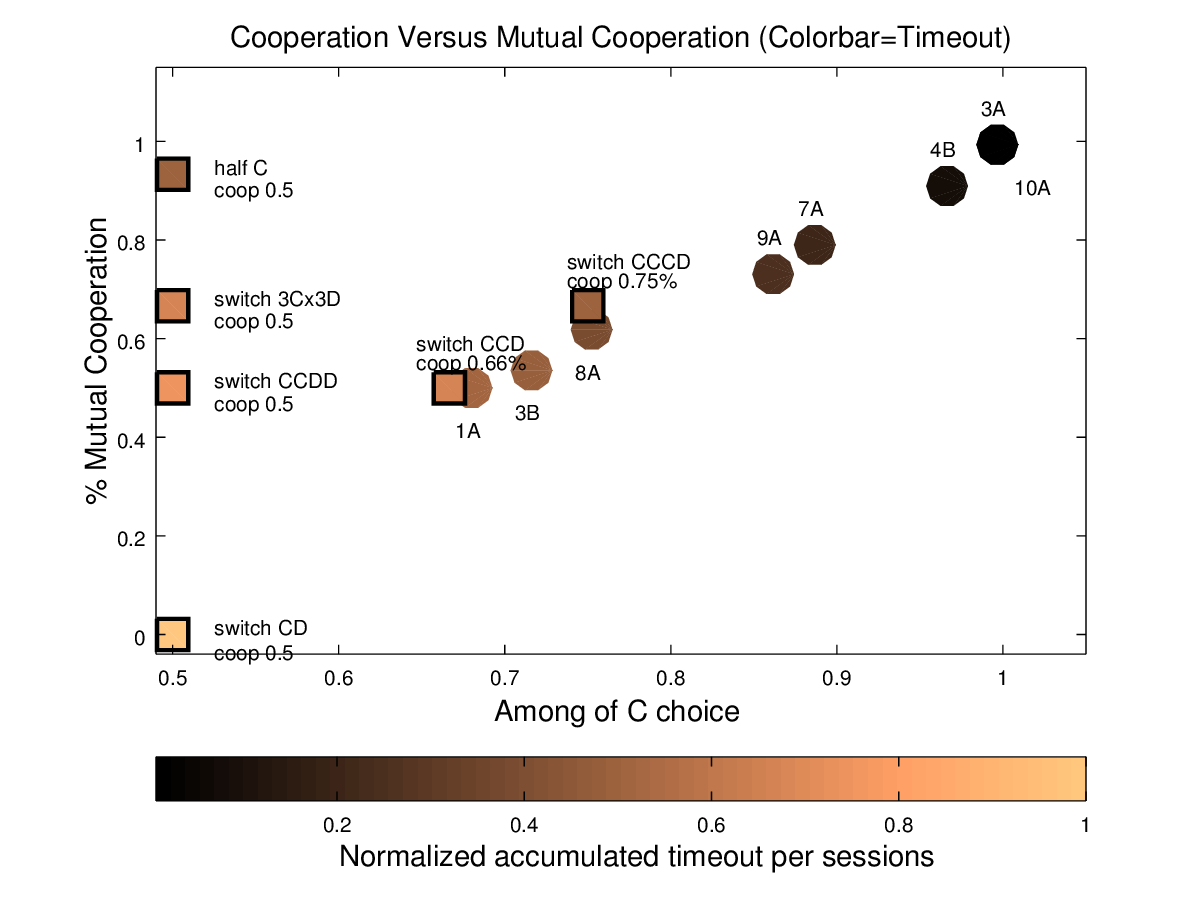
\includegraphics[width=0.45\columnwidth]{/home/guille/Documents/experimento/Experimento---iPD/ExtraerDatos/figura_iPD_1_2_9s_13s/fig_finales/cooperacionVscoopMutua_delay_sinrandom}

\label{fig_coopMutua}}\hfill{}\subfloat[Total reward versus cooperation choice]{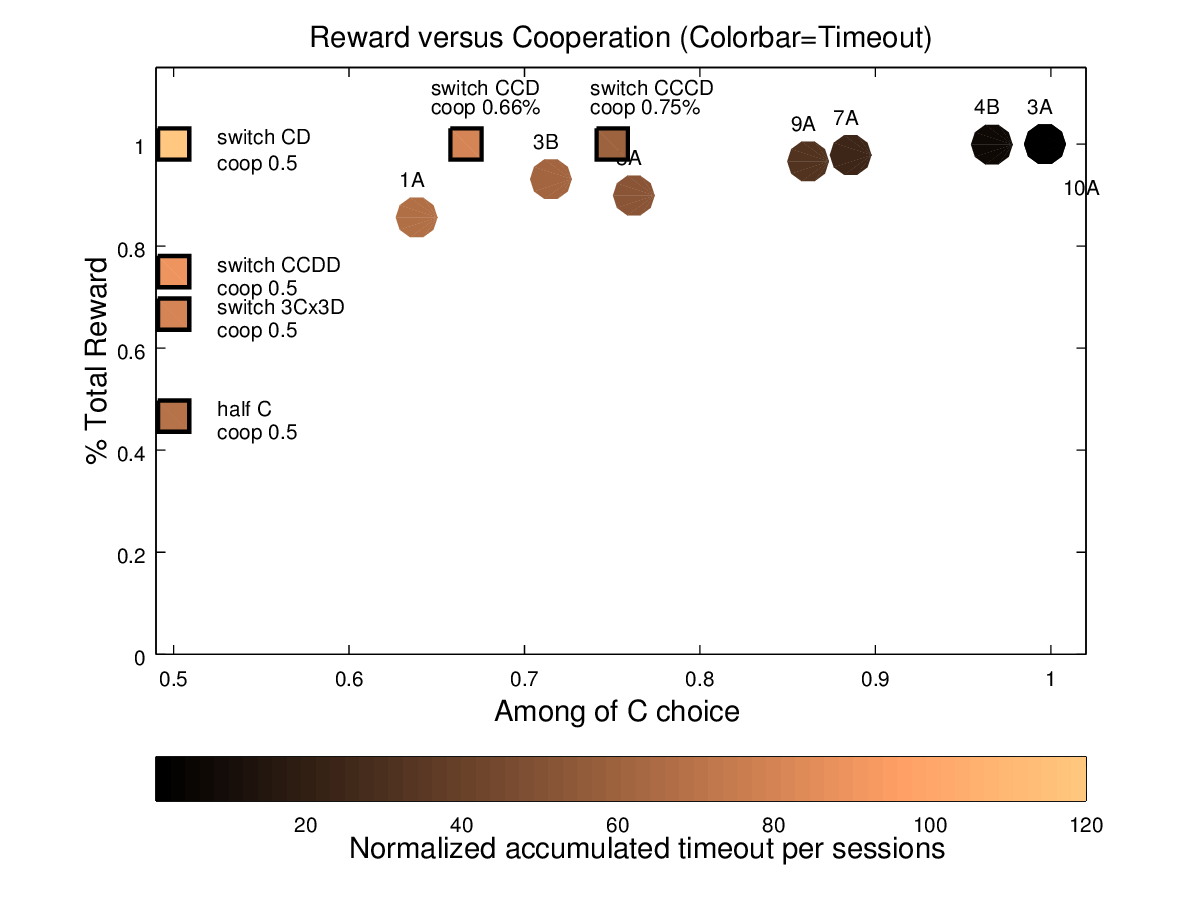
\includegraphics[width=0.45\columnwidth]{/home/guille/Documents/experimento/Experimento---iPD/ExtraerDatos/figura_iPD_1_2_9s_13s/fig_finales/cooperacionVsReward_delay_sinrandom}



\label{fig_rewardVScoop}}\hfill{}

\hfill{}\subfloat[Total Reward versus accumulated timeout]{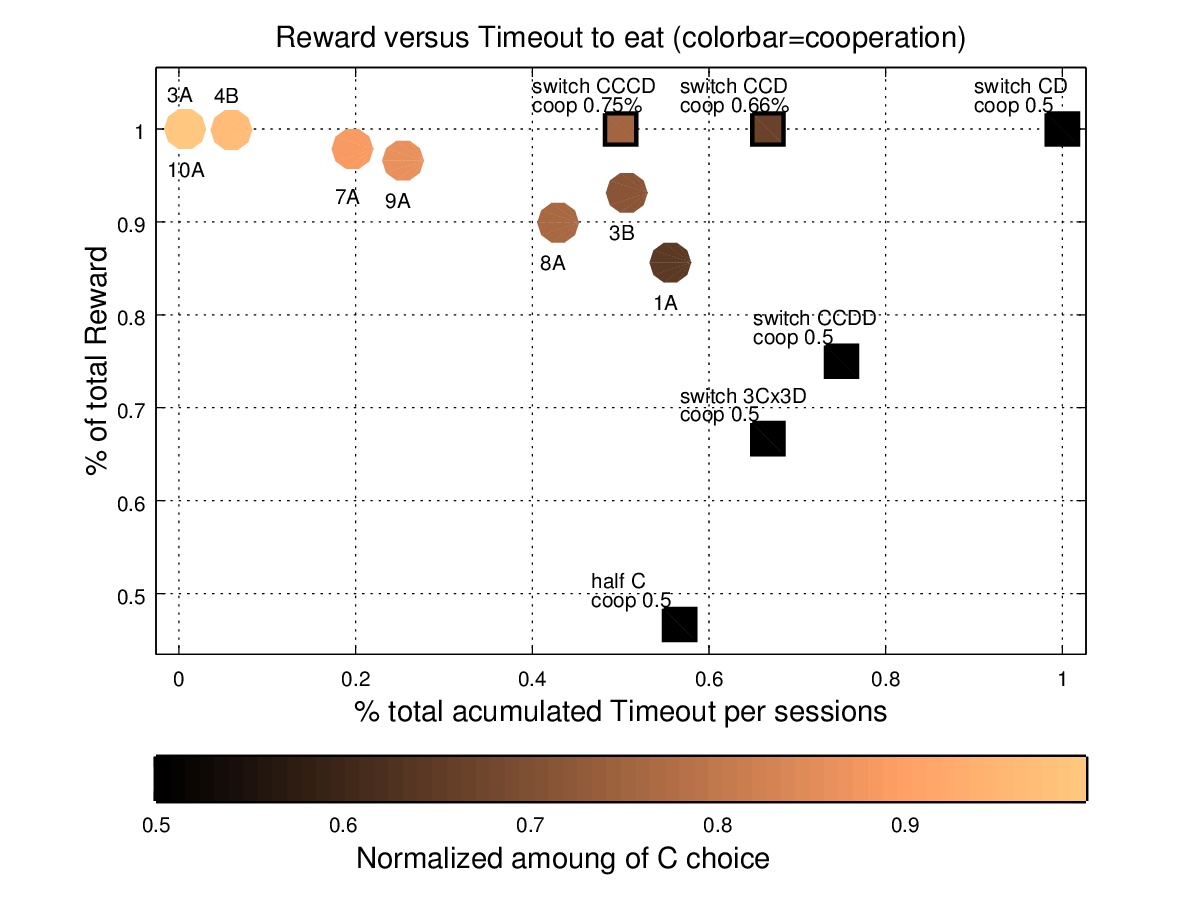
\includegraphics[width=0.45\columnwidth]{/home/guille/Documents/experimento/Experimento---iPD/ExtraerDatos/figura_iPD_1_2_9s_13s/fig_finales/alimentoVstimeout_cooperation}



\label{fig_reward VS timeout}}\hfill{}\subfloat[Preference Coefficient.]{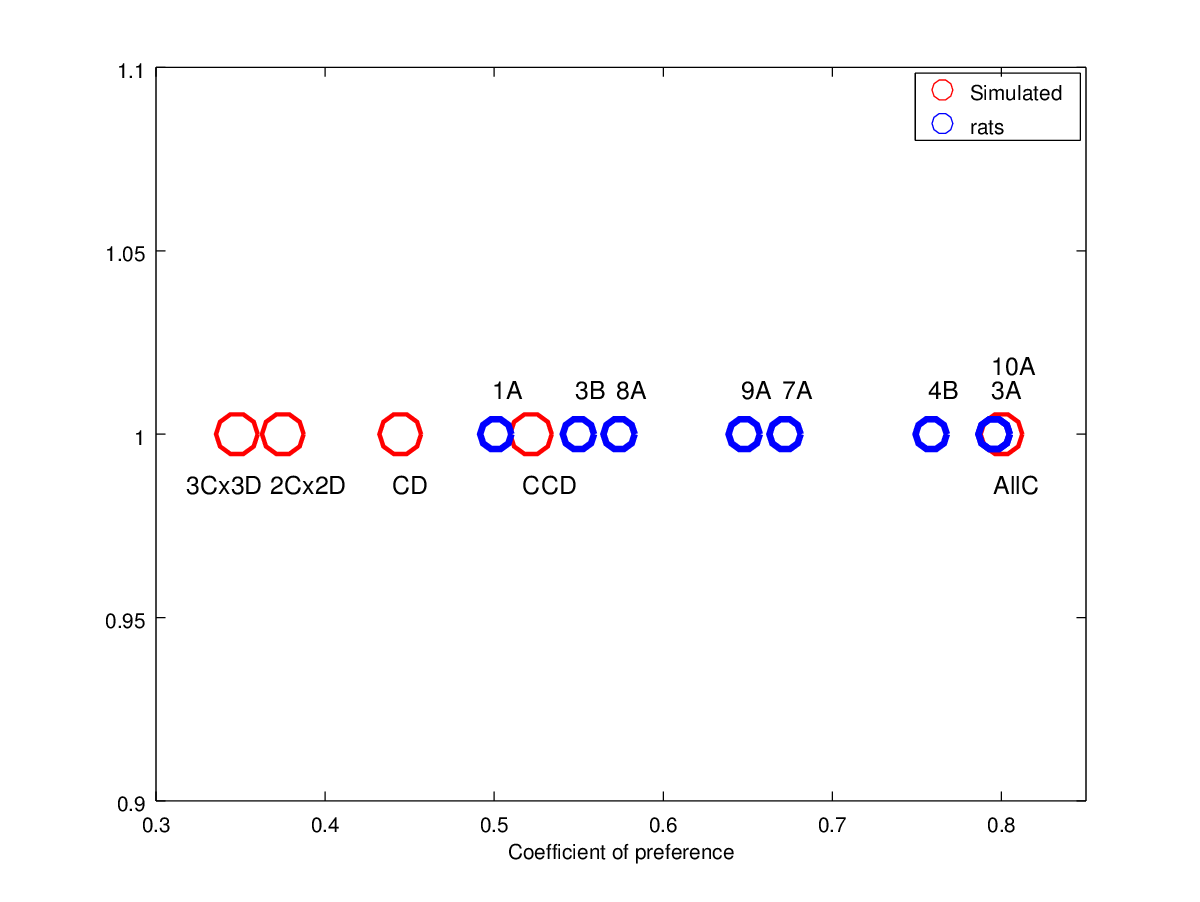
\includegraphics[width=0.45\columnwidth]{/home/guille/Documents/experimento/Experimento---iPD/ExtraerDatos/figura_iPD_1_2_9s_13s/fig_finales/coefficientOfPreference2}



\label{fig_CoeffPreference}}\hfill{}

\caption{{\scriptsize{}There experiment's result was computed from last ten
session pool data set. \ref{fig_coopMutua}) The graph of Mutual cooperations
versus cooperation show that the subject (filled circle) had a directly
proportional relationship, mutual cooperate less when cooperate less.
The color bar represent average accumulated punishment (second) that
each subject obtain per sessions and also is drive by same relationship
respect . The square represent theoretical behaviors. \ref{fig_rewardVScoop})
The graph show the percentage of cooperation versus total reward.
All animals obtain more that 80\% of total reward per session. The
simulated agent (filled square) help to understand the strategies
used by animals. \ref{fig_reward VS timeout}) The figure show the
relation between rewards and timeout punishment, the color bar point
out the level cooperation choice. Since the graph we observe that
the highest reward corresponds to the subject with less accumulated
timeout punishment and they also have the highest cooperation choice
level. \ref{fig_CoeffPreference}) The Coefficient of preference is
the quotient between reward and punishment that each rat got as result
to used one strategy. the blue circle are the coefficient of preference
per rat and the size are the level of cooperation. The red circle
are the coefficient for the simulated rats. All rats has a strategy
more cooperative than the simulated rats with alternated ``CD''
strategy.}}
\end{figure}


The reciprocate strategy is mainly defined by the probability of mutual
cooperation. Thus we made a graph of Mutual cooperations versus cooperation
and saw that exist a directly proportional relationship between them,
if mutual cooperate does down then the cooperate choice goes down,
the correlation coefficient was $0.996$(\emph{Pearson coefficient}).
It result point out that both variable are related. See figure \ref{fig_coopMutua}.
The color bar represent average accumulated punishment (second) that
each subject obtain per sessions in the last ten session and also
is drive by same relationship respect both mutual cooperation or cooperation
choice, the correlation coefficient was $-0.998$ and $-0.935$ respectively.
When cooperation up, the punishment down. In the figure, the square
point represent theoretical simulated behaviors and used to compare
the real average rat behavior respect to these repetitive simulated
agent. We created the follow behaviors: \emph{1�)``switch CD''}
in which the theoretical subject always alternated between cooperate
(C) lever and defect (D) lever; 2�) ``switch CCDD'' is similar to
the previous but the subject choose consecutively 2 time the same
lever and then change to the other lever and repeat the action; 3�)
``switch 3C3D'' the subject choose consecutively 3 time the same
lever and then change; 4�) ``half C'' the subject choose the same
lever until the middle of session, then change and doesn't change
at the end; 5�) ``switch CCD'' in which choose 2 time C lever and
then choose only a time the D lever and go back to the previous C
lever and repeat the action. 6�) ``switch CCCD'' is similar to the
previous but the subject choose 3 time C lever. These simulations
allow to visualize specific behavior and make assumptions about rats
behaviors.

All rats got the high level of reward, over 80\%, despite of the dispersion
of mutual cooperation data, fig. \ref{fig_reward VS timeout}. Since
the simulated agent (filled square) are used to understand the kind
of strategy used by the rats, we observe that the rats after make
a defeat choice trend to learned that they have to back to cooperate
choice. The rats of the group with lowest mutual cooperation level
are near the simulated agent with ``Switch CCD'' and ``Switch CCCD''
behaviors. 

Relating rewards with punishment level we develop a coefficient that
named Preference, and it can help to understand the preference for
choose lever C, figure \ref{fig_CoeffPreference}. The left side of
``CD'' there are the simulated agent with strategies fewer cooperative,
choose D more than one time, consecutively. And the right side of
``CD'' represent the strategies in which choose C more than one
time, consecutively, and only a time D.


\subsubsection{Second Phase: reversion}

The second phase experiment was developed to understand if the behaviors
exhibit by the rats was either learned through the experience into
the iPD game or was simply the choice of one lever, cooperation, by
chance. If was by chance and now levers position change, the rats
is going to choose same lever. We used four rats that got the best
score in the previous experiment. In this phase, the levers order
was inverted, i.e. if in previous experiment the lever meant cooperate,
it became to defeat lever. We procedures in the same way as in the
first experiment. The sessions duration per rat were: {\scriptsize{}3A/52;
7A/52; 9A/52; 10A/24;}. The means of cooperation from the last 10
session is showed in the figure \ref{fig1_REV_meansAnd significance-1}
and the asterisk denote the rats with some fix strategy and that it
is different to the random strategy.

\begin{figure}
\begin{centering}
{\scriptsize{}\hfill{}}\subfloat[{\scriptsize{}Cooperation mean}]{\begin{centering}
{\scriptsize{}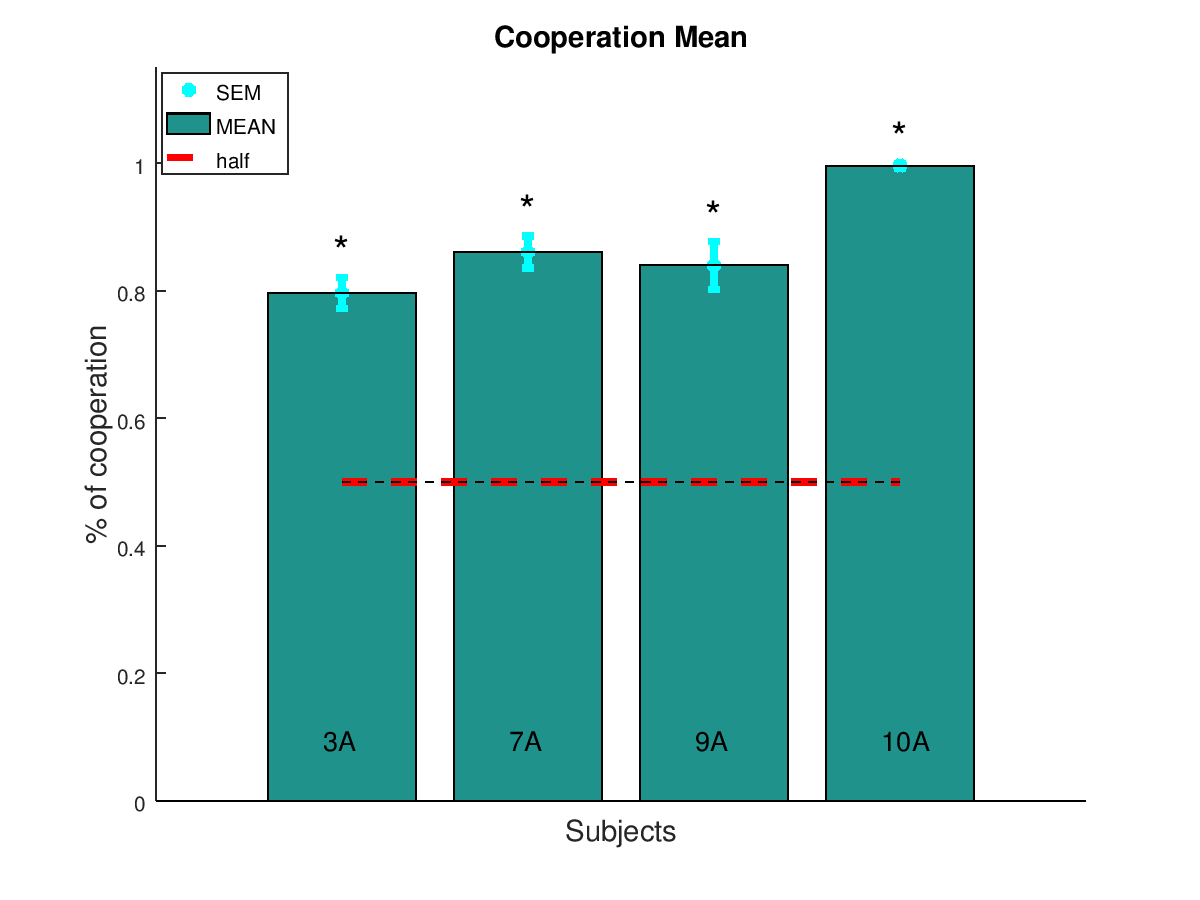
\includegraphics[width=0.45\textwidth]{/home/guille/Documents/experimento/Experimento---iPD/ExtraerDatos/figura_iPD_1_2_9s_13s/fig_finales/cooperation_mean_with_significant_reversion}}
\par\end{centering}{\scriptsize \par}

\begin{centering}
{\scriptsize{}}
\par\end{centering}{\scriptsize \par}

\centering{}{\scriptsize{}\label{fig1_REV_meansAnd significance-1}}}{\scriptsize{}\hfill{}}\subfloat[Reward mean ]{\begin{centering}
{\scriptsize{}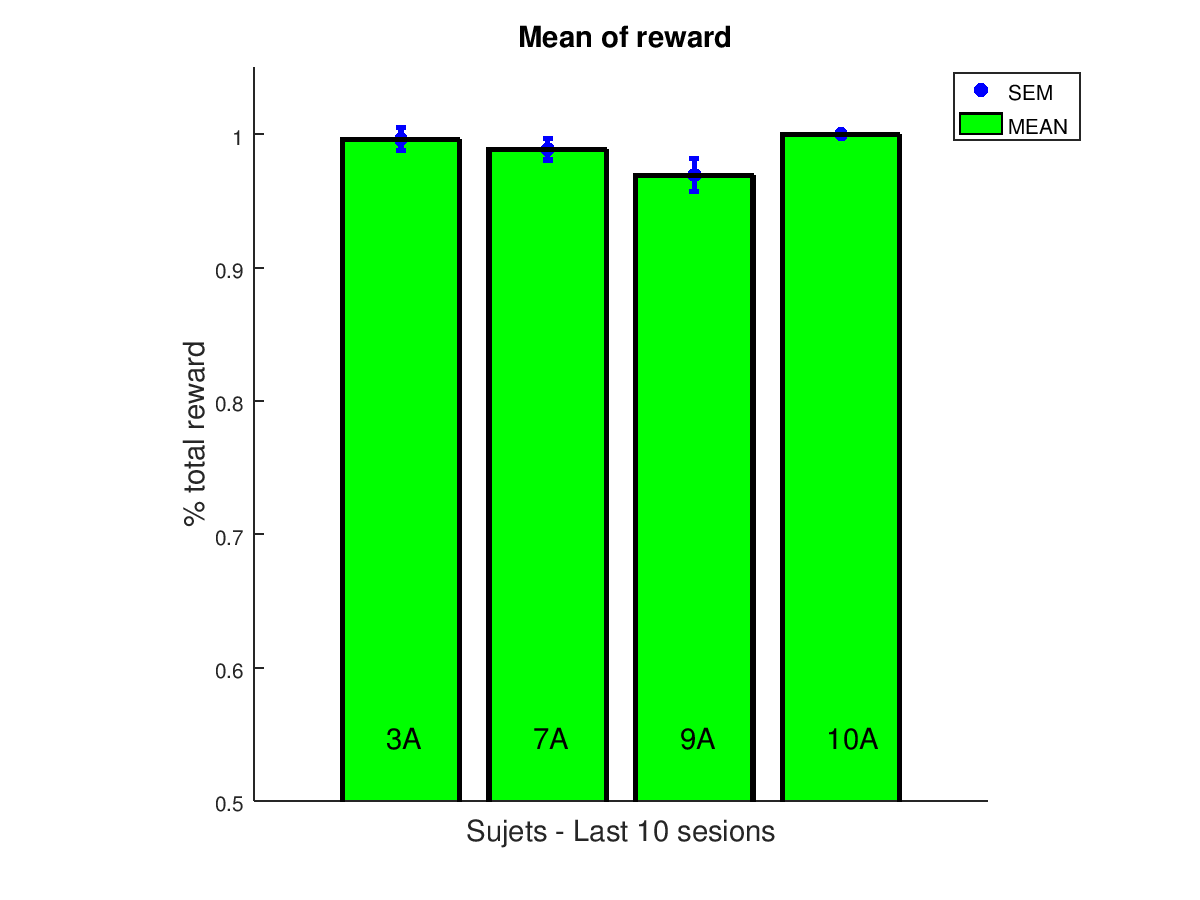
\includegraphics[width=0.45\textwidth]{/home/guille/Documents/experimento/Experimento---iPD/ExtraerDatos/figura_iPD_1_2_9s_13s/fig_finales/mean_reward_reversion}}
\par\end{centering}{\scriptsize \par}

\begin{centering}
{\scriptsize{}}
\par\end{centering}{\scriptsize \par}

\centering{}{\scriptsize{}\label{fig_REV_meanReward-1-1}}}{\scriptsize{}\hfill{}}
\par\end{centering}{\scriptsize \par}

\begin{centering}
{\scriptsize{}\hfill{}}\subfloat[{\scriptsize{}Timeout mean}]{\begin{centering}
{\scriptsize{}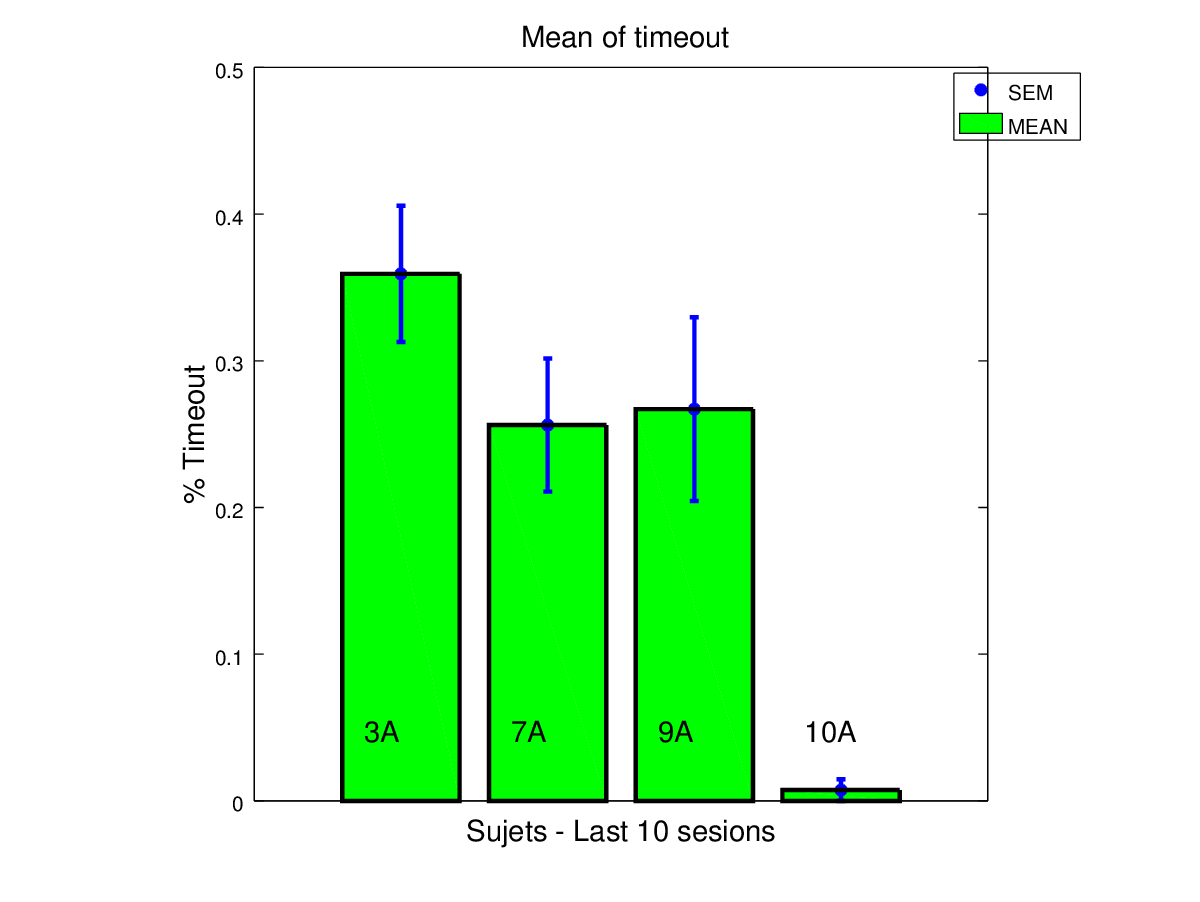
\includegraphics[width=0.45\textwidth]{/home/guille/Documents/experimento/Experimento---iPD/ExtraerDatos/figura_iPD_1_2_9s_13s/fig_finales/mean_timeout_reversion}}
\par\end{centering}{\scriptsize \par}

\begin{centering}
{\scriptsize{}}
\par\end{centering}{\scriptsize \par}

\centering{}{\scriptsize{}\label{fig1_REV_meansTimeout}}}{\scriptsize{}\hfill{}}\subfloat[Evolution of cooperation]{\begin{centering}
\textcolor{red}{\large{}FALTA}{\scriptsize{}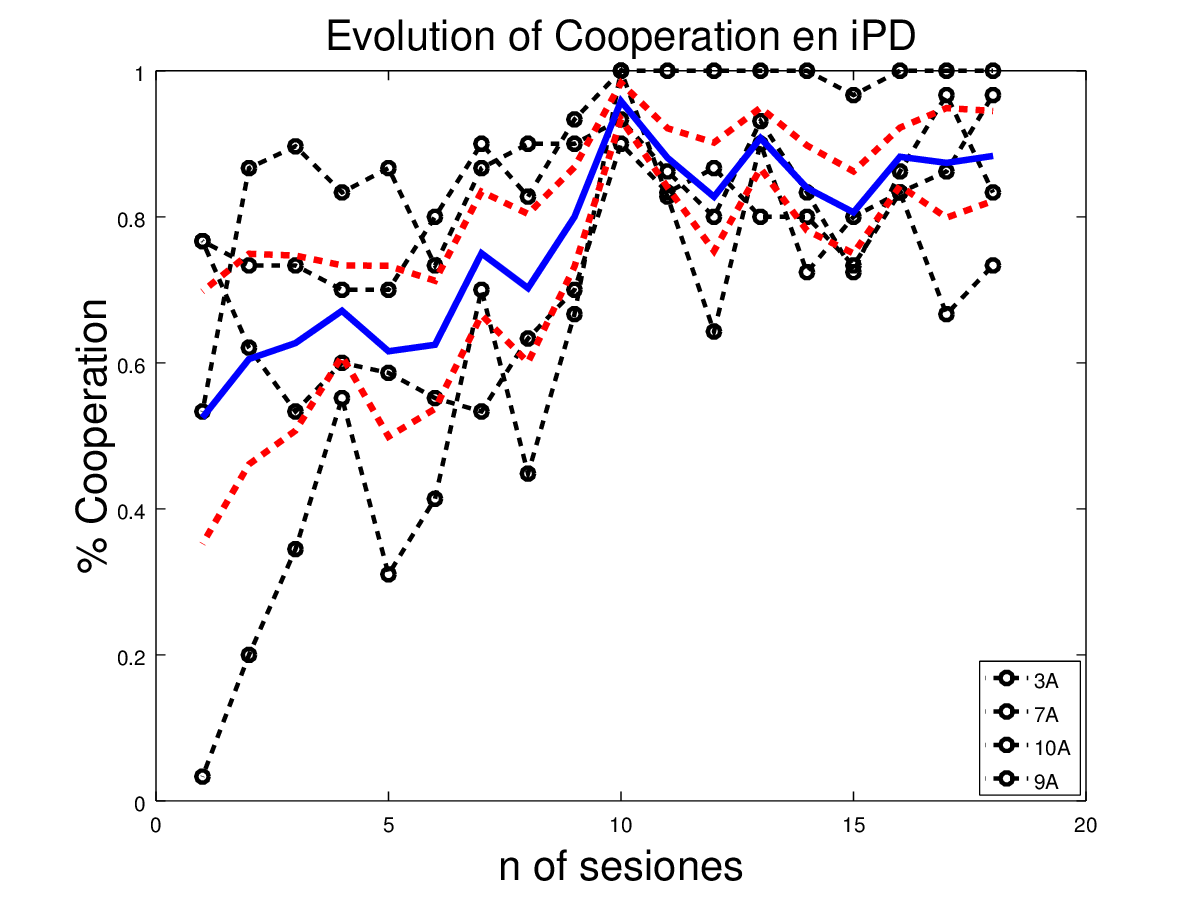
\includegraphics[width=0.45\textwidth]{/home/guille/Documents/experimento/Experimento---iPD/ExtraerDatos/figura_iPD_1_2_9s_13s/fig_finales/cooperation_mean_sem_last18session_Reversion}}
\par\end{centering}{\scriptsize \par}

\begin{centering}
{\scriptsize{}}
\par\end{centering}{\scriptsize \par}

\centering{}{\scriptsize{}\label{fig_REV_evolution_coop_rev}}}{\scriptsize{}\hfill{}}
\par\end{centering}{\scriptsize \par}

{\scriptsize{}\caption{{\scriptsize{}\ref{fig1_REV_meansAnd significance-1})}\textbf{\scriptsize{}Mean
and }{\scriptsize{}$\chi{}^{2}$}\textbf{\scriptsize{}test}{\scriptsize{}:
The rats with 95\% of free feeding body weight played under a matrix
pay-off T=2, R=1,P=4''delay, S=8''delay against a TFT opponent.
We show means of the numbers of times rats chose the cooperate option
($mean\pm s.e.m.$). The Asterix denote when the rat adopted a strategy
that had significant difference from chance strategy ($\chi{}^{2}$
goodness of fit test with bonferroni corrected, p>0.125). The rats
without significant difference did not surpass 0.5 probability of
cooperation. \ref{fig_REV_meanReward-1-1}) }\textbf{\scriptsize{}Means
of reward.}{\scriptsize{} Bar line shows the mean of obtained reward
per session over the last 10 session ($mean\pm s.e.m.$). The rats
with random strategy (not chi-square significant) obtained the lowest
level of reward, below 75\% of total reward. \ref{fig1_REV_meansTimeout})
Means of Timeout is the punishment that each rat got by develop a
learned strategy. \ref{fig_REV_evolution_coop_rev}) Evolution of
cooperation choice from a data set with the last 18 sessions. The
blue and continuous and thicker line is the means per session of the
group and the dotter line is the standard error of the mean ($mean\pm sem=[0.866\pm0.015]$over
the las ten sessions). The vertical dotter line mark the pool of data
that was used to analyse the strategies adopted by the rats. }}
}
\end{figure}


\begin{table}
\label{table_REV_meanAndstrategies-1}\caption{{\scriptsize{}We show the mean of cooperation and the probabilities
of cooperation given each outcomes. The $\chi^{2}$goodness of fit
with bonferroni correction was performed used a theorical frecuency
of 0.5. The significance value show the subject that developed a specific
strategy. The subject underlined and in blue text color had significant
different respect random strategy. }}


{\scriptsize{}}%
\begin{tabular}{|c|c|c|c|c|c|c|c|}
\hline 
 & {\scriptsize{}Mean} & \multicolumn{4}{c|}{Strategies} &  & \tabularnewline
\cline{1-1} \cline{3-8} 
{\scriptsize{}Subject} & {\scriptsize{}cooperation} & {\tiny{}$p(c|T)$} & {\tiny{}$p(c|R)$} & {\tiny{}$p(c|P)$} & {\tiny{}$p(c|S)$} & {\tiny{}$\chi_{bonferroni}^{2}$} & {\tiny{}$p<0.0125$}\tabularnewline
\hline 
\hline 
\textbf{\textcolor{blue}{\tiny{}3A}} & {\tiny{}$0.796$} & {\tiny{}$0.89130$} & \textbf{\tiny{}$0.794$} & {\tiny{}$1$} & {\tiny{}$0.778$} & {\tiny{}$113.336$} & \textcolor{blue}{\tiny{}$0.0000$}\tabularnewline
\hline 
\textbf{\textcolor{blue}{\tiny{}7A}} & {\tiny{}$0.861$} & {\tiny{}$0.875$} & \textbf{\tiny{}$0.889$} & {\tiny{}$1$} & {\tiny{}$0.719$} & {\tiny{}$117.942$} & \textcolor{blue}{\tiny{}$0.0000$}\tabularnewline
\hline 
\textbf{\textcolor{blue}{\tiny{}9A}} & {\tiny{}$0.840$} & {\tiny{}$0.677$} & \textbf{\tiny{}$0.871$} & {\tiny{}$1$} & {\tiny{}$0.767$} & {\tiny{}$98.041$} & \textcolor{blue}{\tiny{}$0.0000$}\tabularnewline
\hline 
\textbf{\textcolor{blue}{\tiny{}10A}} & {\tiny{}0.996} & {\tiny{}$1$} & \textbf{\tiny{}$1$} & {\tiny{}$0.000$} & {\tiny{}$1$} & {\tiny{}$200.000$} & \textcolor{blue}{\tiny{}$0.0000$}\tabularnewline
\hline 
\end{tabular}
\end{table}


,

,

\begin{figure}
\subfloat[{\scriptsize{}Mean of cooperation and means of transition vector}]{\begin{centering}
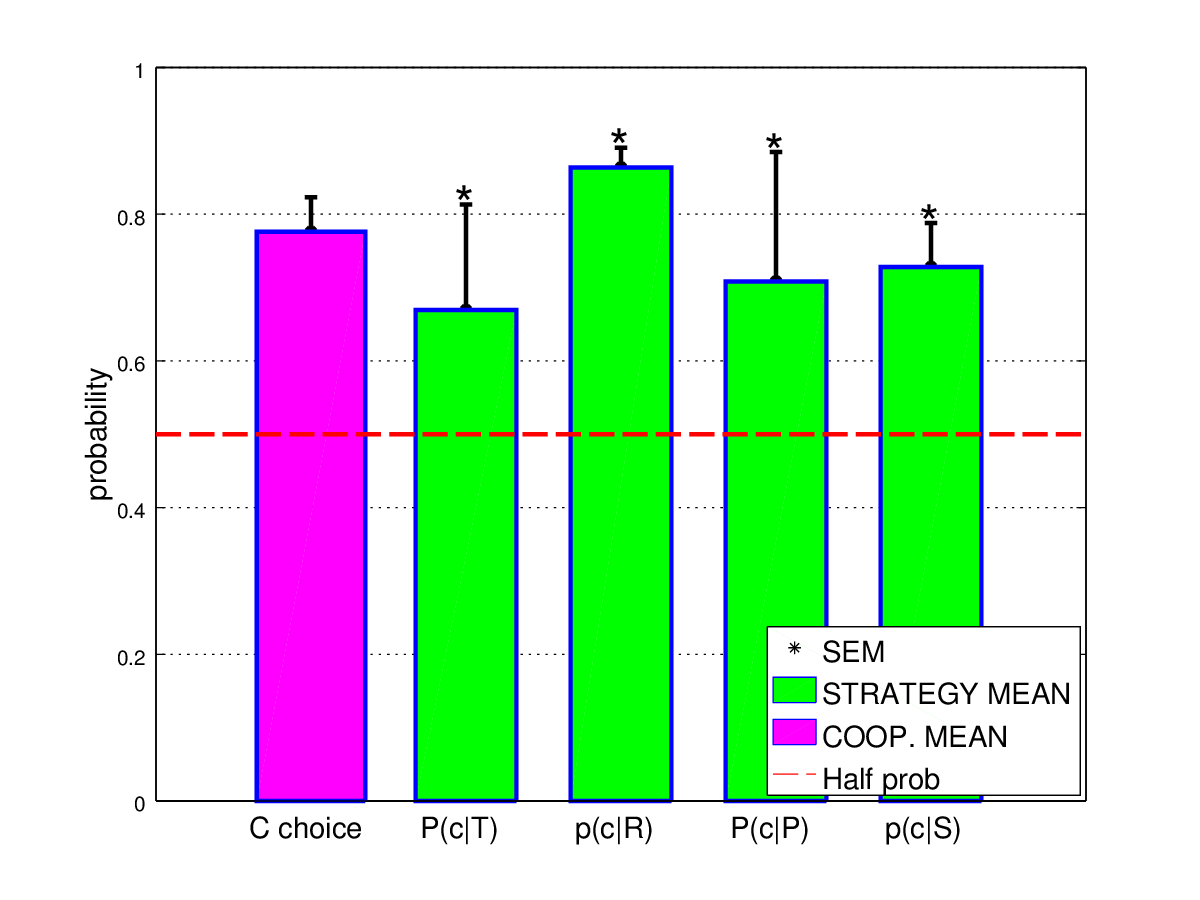
\includegraphics[width=0.45\columnwidth]{/home/guille/Documents/experimento/Experimento---iPD/ExtraerDatos/figura_iPD_1_2_9s_13s/fig_finales/mean_cooperation_and_strategy_reversion}
\par\end{centering}

\begin{centering}

\par\end{centering}

\label{fig_REV_meanC_strategy-1}}\hfill{}\subfloat[{\scriptsize{}Outcomes rates over the last ten sessions.}]{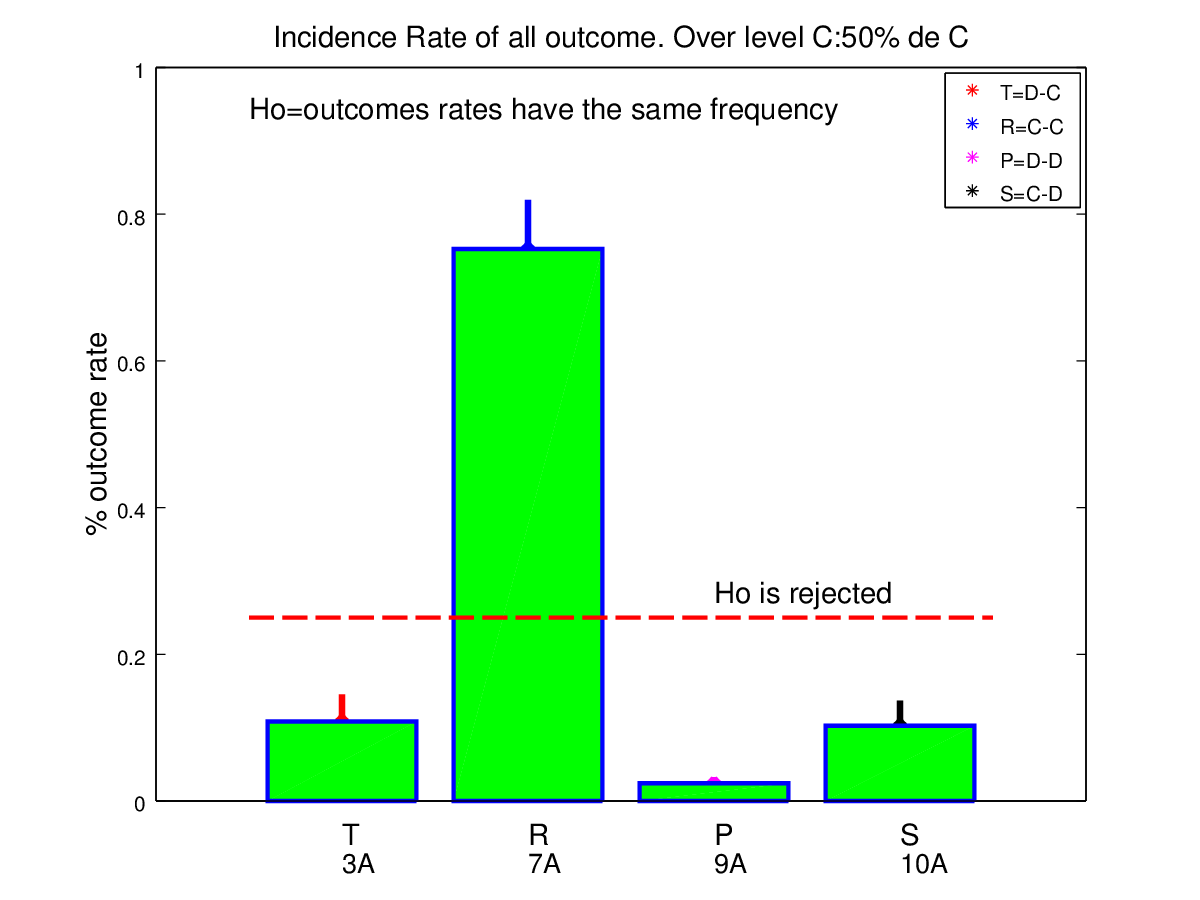
\includegraphics[width=0.45\columnwidth]{/home/guille/Documents/experimento/Experimento---iPD/ExtraerDatos/figura_iPD_1_2_9s_13s/fig_finales/outcomeRate_overLevel_reversion}



\label{fig_REV_outcomes rate-1}}

\hfill{}\subfloat[{\scriptsize{}Markov chain graph of four state}]{\begin{centering}
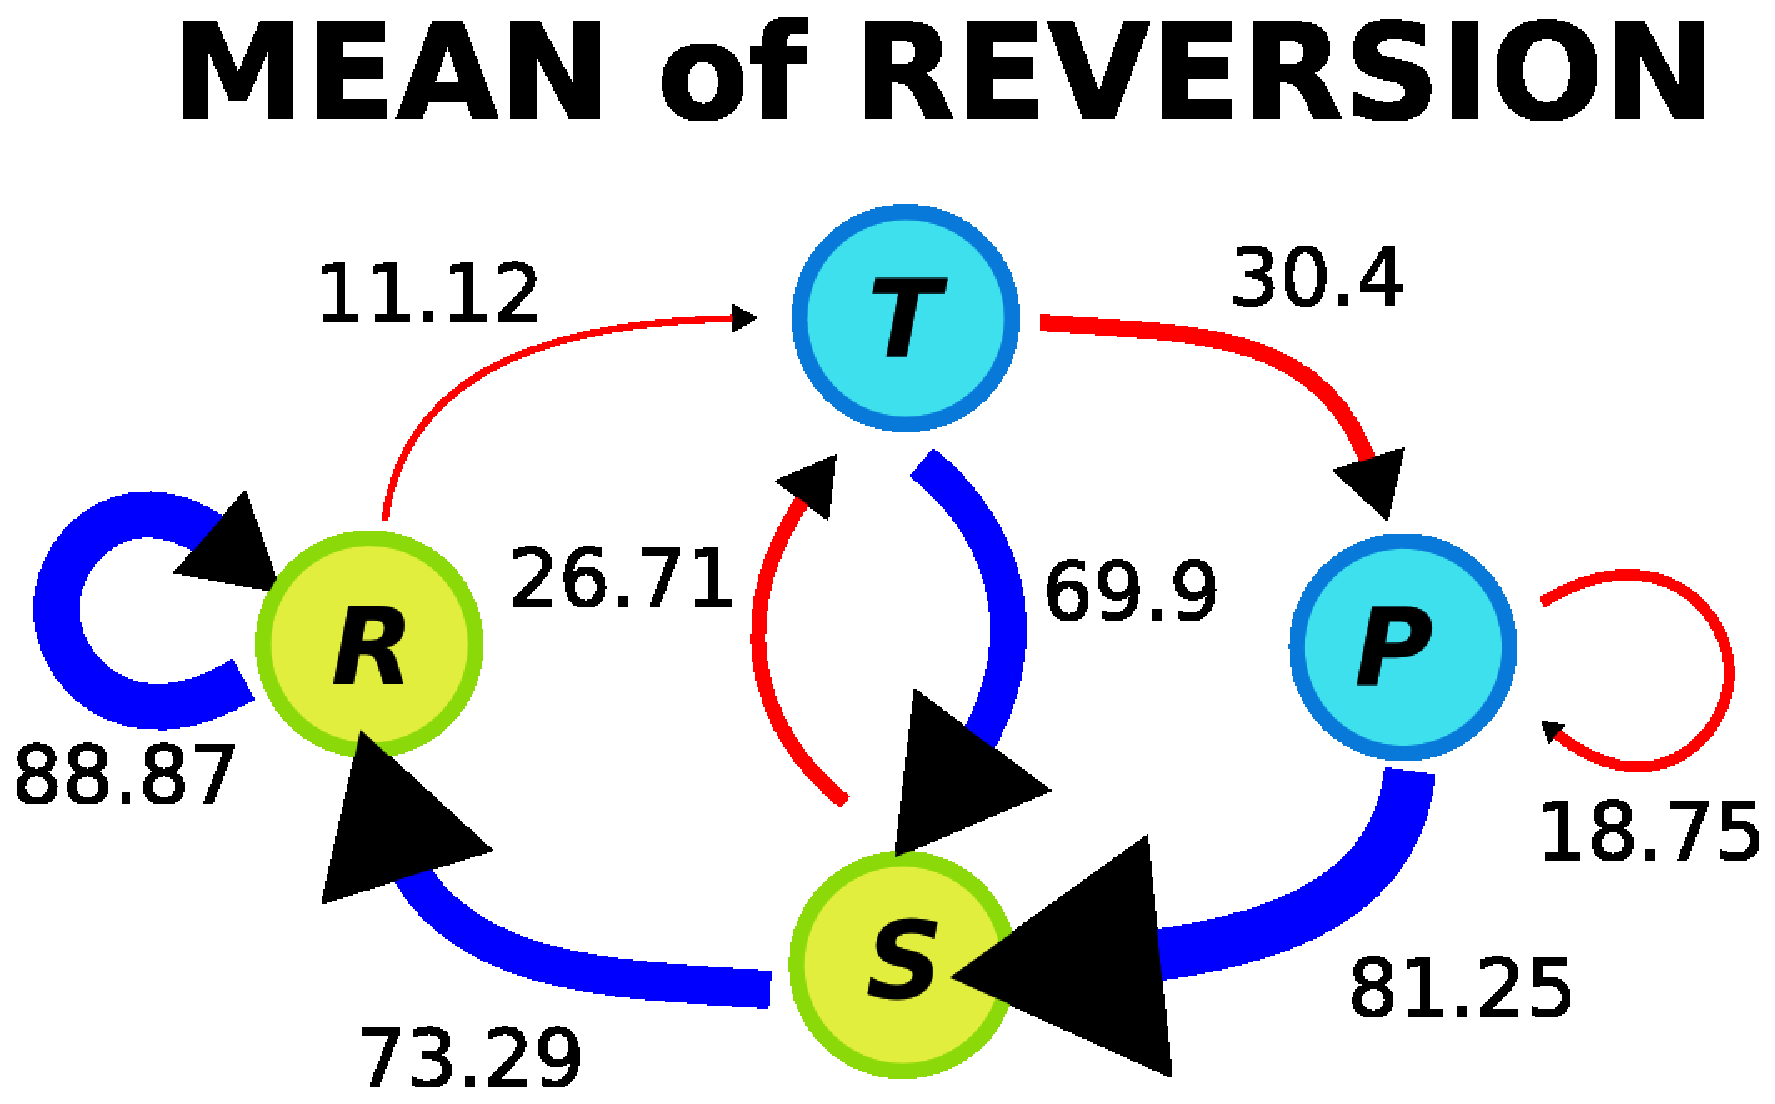
\includegraphics[width=0.4\columnwidth]{/home/guille/Documents/experimento/Experimento---iPD/ExtraerDatos/figura_iPD_1_2_9s_13s/fig_finales/markov_4estados_mean_reversion}
\par\end{centering}



\label{fig_REV_4state_markovChain-1}}\hfill{}\subfloat[Markov chain graph of two state]{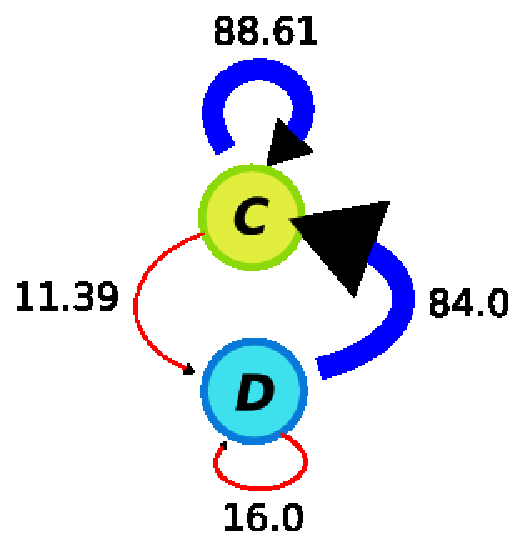
\includegraphics[width=0.3\columnwidth]{/home/guille/Documents/experimento/Experimento---iPD/ExtraerDatos/figura_iPD_1_2_9s_13s/fig_finales/g33959}



\label{fig_REV_2state_markovChain-1}}\hfill{}

\caption{{\scriptsize{}\ref{fig_REV_meanC_strategy-1}) Mean of cooperation
over not random strategy rats (8 rats) was performed and the measured
is shown on the first magenta bar ($mean=0.852$ and $s.e.m.=\pm0.0482$
). The next four green bars represent the mean strategy over the group
and each bar agree with the transition vector,$v=[0.794,0.856,0.801,0.890]$.
The asterisk indicates significant difference respect the half probability
of chose cooperation lever and we tested by $\chi{}^{2}$ goodness
of fit with theory frequency 0.5. \ref{fig_REV_outcomes rate-1})
The bar graph shows the outcomes rates and suggest that R outcomes
had very high incidence in the experiment over the last 10 sessions.
. We found significant difference between outcomes (Friedman's ANOVA
test was performed with bonferroni correction ($\alpha=0.0125,p>3.3e-5;\chi^{2}=23.4$)
and Multiple pairwise comparison's using Nemeyi's procedure ). \ref{fig_REV_4state_markovChain-1}
and \ref{fig_REV_2state_markovChain-1}) Graph of Markov chain of
four and two state, in which the arrow represent the transition probability
between outcomes. A blue arrow signalized when the subject chose cooperate
lever given the las outcome and a red arrow signalized when it chose
defect lever. The words mean temptation (T), mutual cooperation (R),
punishment (P) and sucker (S). Pay atemption that the arrows width
are proportional to the transition probability. }}
\end{figure}


,

,

\begin{figure}
\hfill{}\subfloat[Mutual Cooperation versus cooperation choice ]{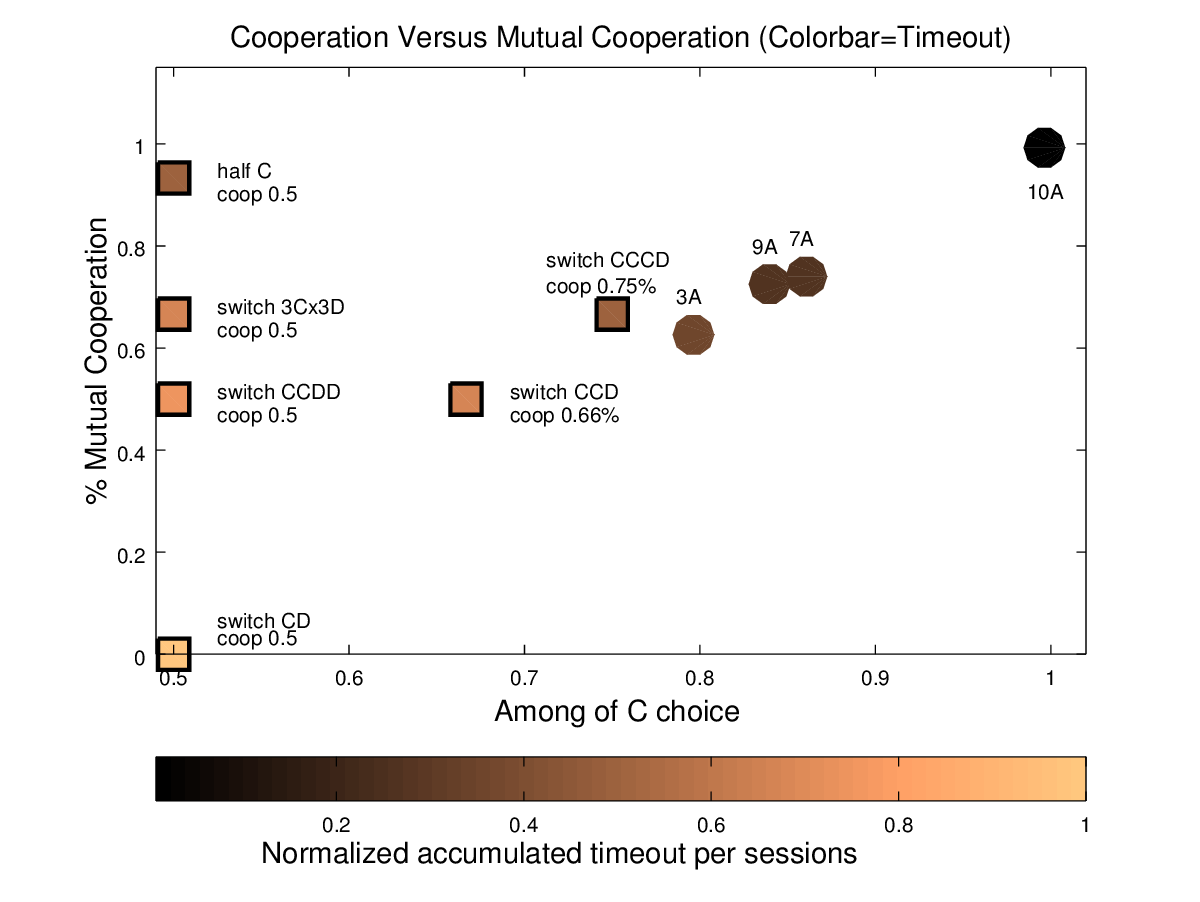
\includegraphics[width=0.45\columnwidth]{/home/guille/Documents/experimento/Experimento---iPD/ExtraerDatos/figura_iPD_1_2_9s_13s/fig_finales/cooperacionVscoopMutua_delay_Reversion}

\label{fig_REV_coopMutua}}\hfill{}\subfloat[Total reward versus cooperation choice]{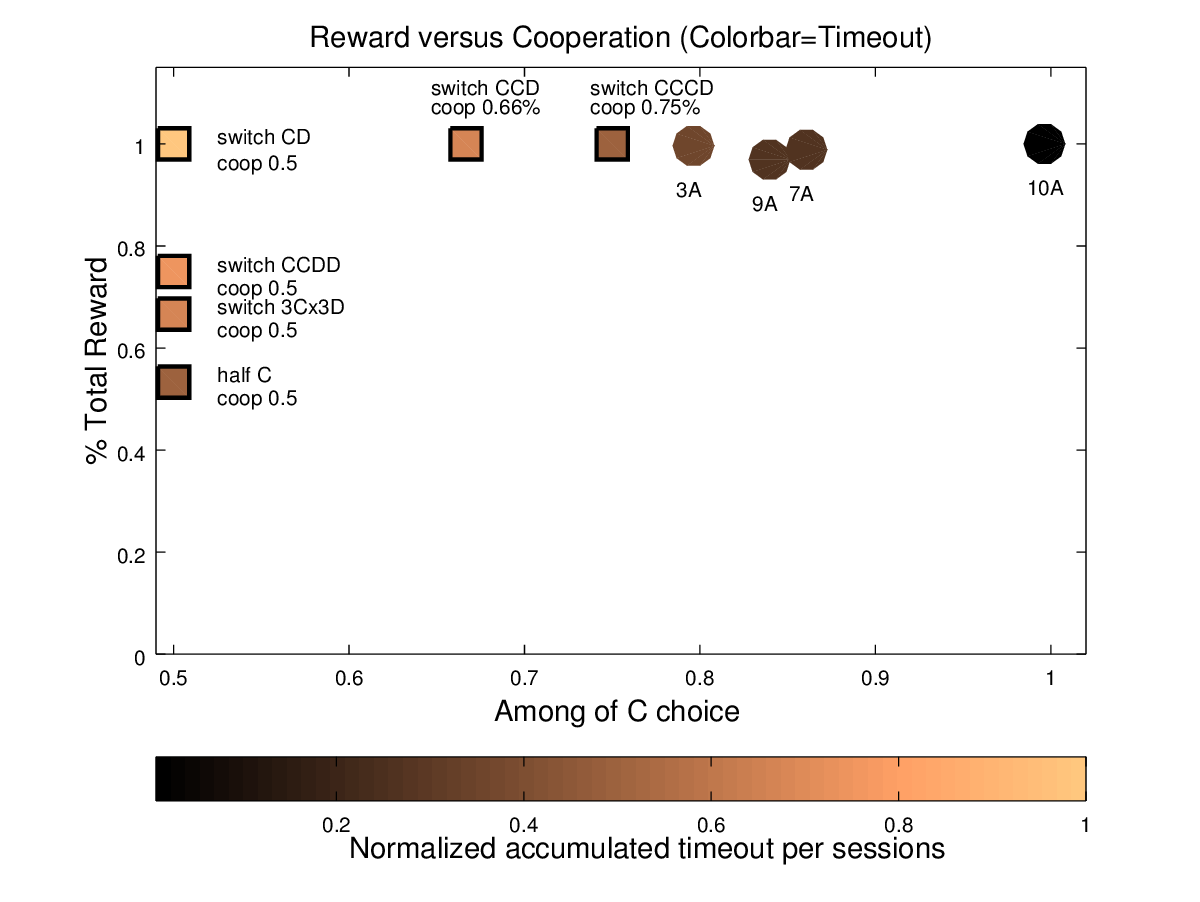
\includegraphics[width=0.45\columnwidth]{/home/guille/Documents/experimento/Experimento---iPD/ExtraerDatos/figura_iPD_1_2_9s_13s/fig_finales/cooperacionVsReward_delay_Reversion}



\label{fig_REV_rewardVScoop}}\hfill{}

\hfill{}\subfloat[Total Reward versus accumulated timeout]{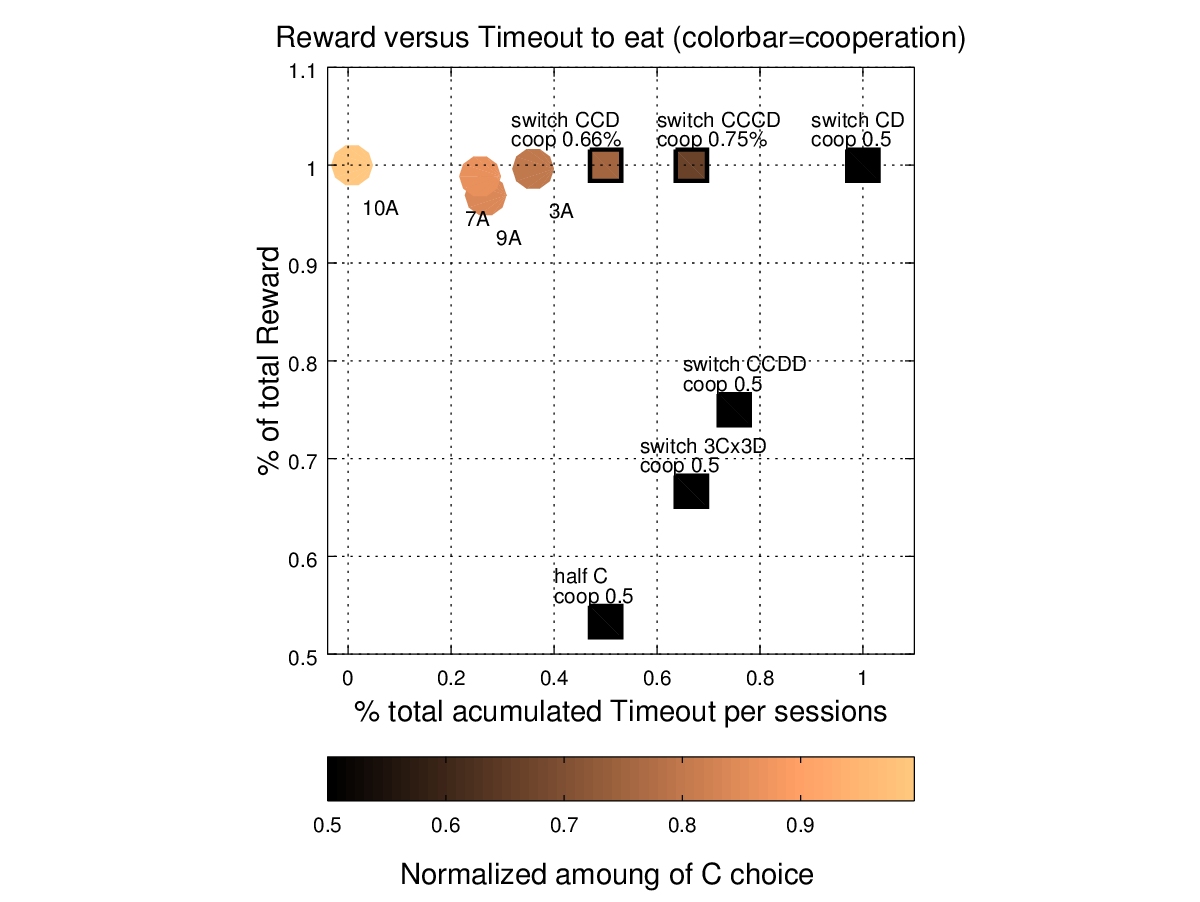
\includegraphics[width=0.45\columnwidth]{/home/guille/Documents/experimento/Experimento---iPD/ExtraerDatos/figura_iPD_1_2_9s_13s/fig_finales/alimentoVstimeout_cooperation_Reversion}



\label{fig_REV_reward VS timeout}}\hfill{}\subfloat[Preference Coefficient.]{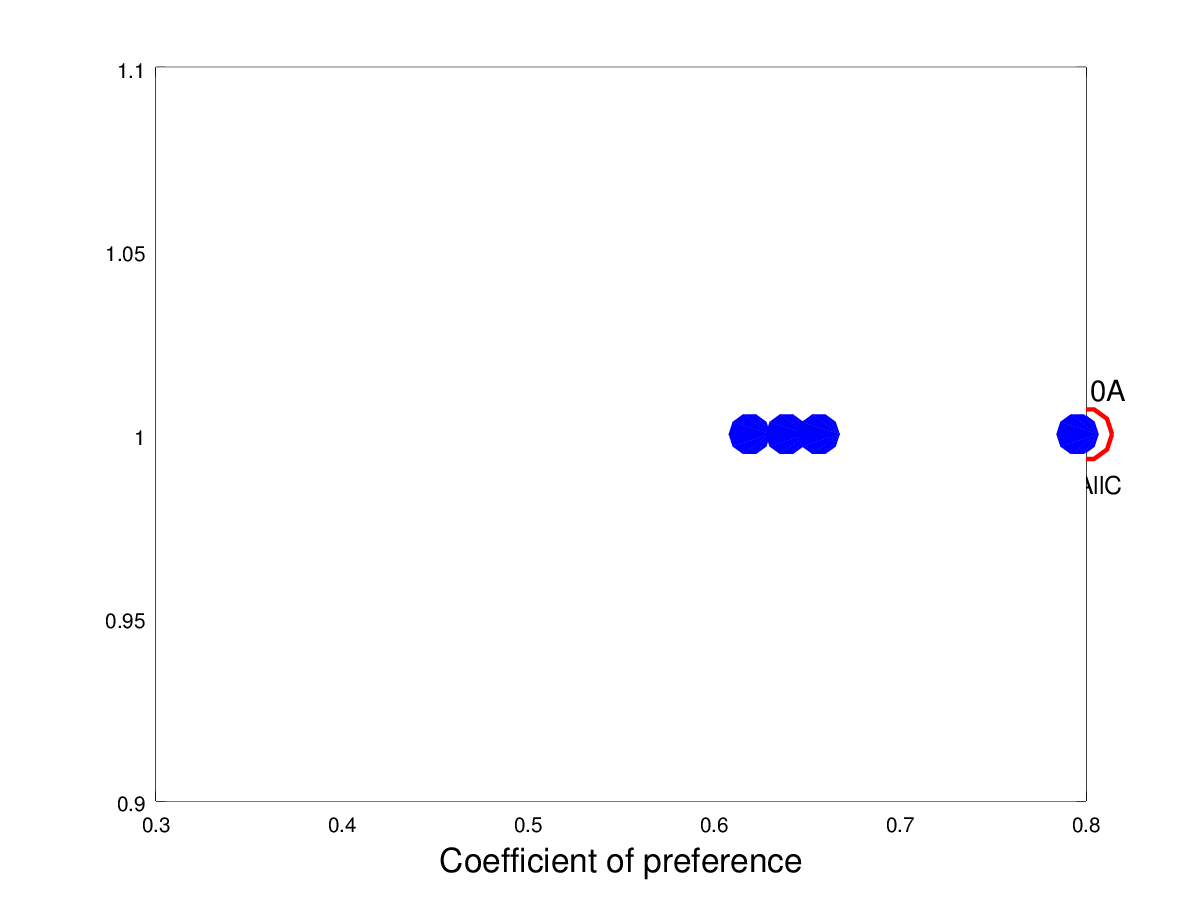
\includegraphics[width=0.45\textwidth]{/home/guille/Documents/experimento/Experimento---iPD/ExtraerDatos/figura_iPD_1_2_9s_13s/fig_finales/coefficientOfPreference_Reversion}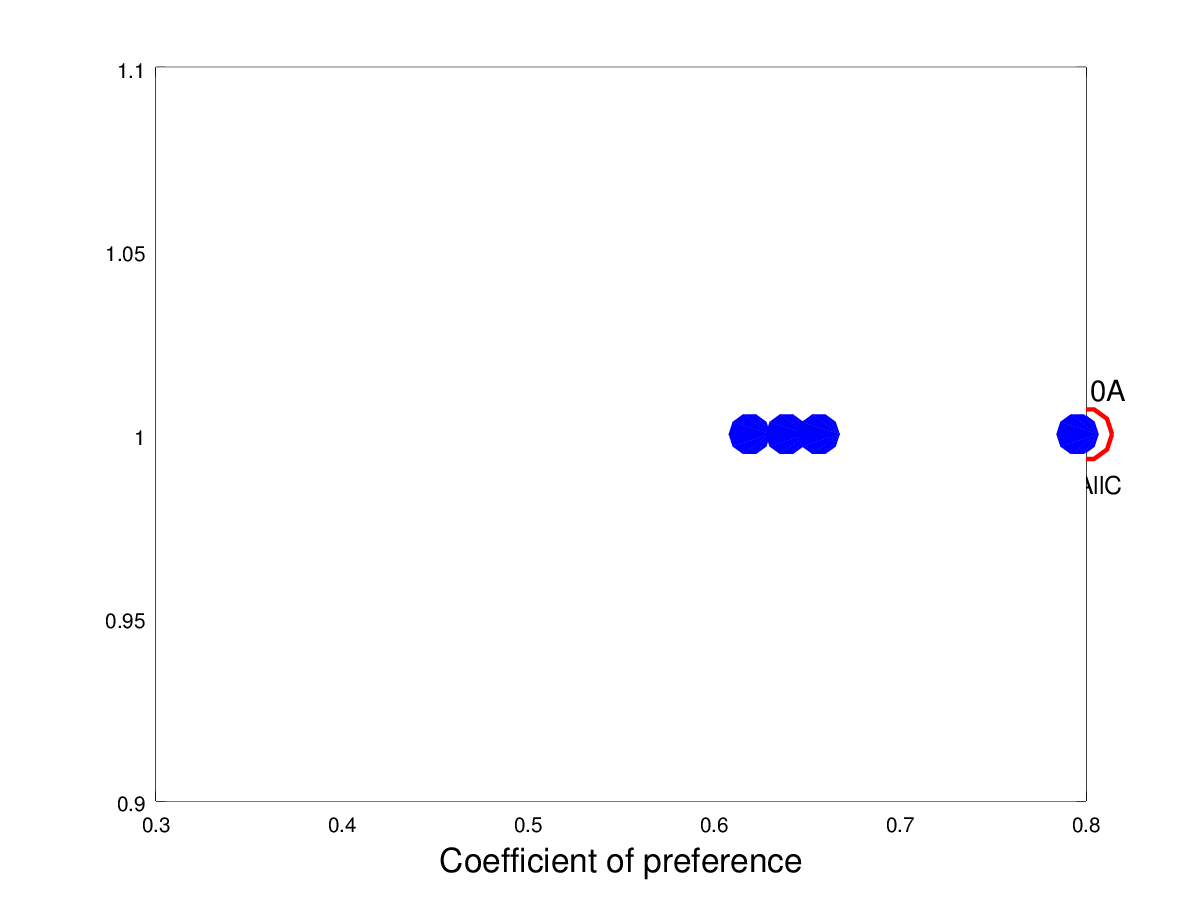
\includegraphics[width=0.45\textwidth]{/home/guille/Documents/experimento/Experimento---iPD/ExtraerDatos/figura_iPD_1_2_9s_13s/fig_finales/coefficientOfPreference_Reversion}



\label{fig_REV_CoeffPreference}}\hfill{}

\caption{{\scriptsize{}There experiment's result was computed from last ten
session pool data set. \ref{fig_REV_coopMutua}) The graph of Mutual
cooperations versus cooperation show that the subject (filled circle)
had a directly proportional relationship, mutual cooperate less when
cooperate less. The color bar represent average accumulated punishment
(second) that each subject obtain per sessions and also is drive by
same relationship respect . The square represent theoretical behaviors.
\ref{fig_REV_rewardVScoop}) The graph show the percentage of cooperation
versus total reward. All animals obtain more that 80\% of total reward
per session. The simulated agent (filled square) help to understand
the strategies used by animals. \ref{fig_REV_reward VS timeout})
The figure show the relation between rewards and timeout punishment,
the color bar point out the level cooperation choice. Since the graph
we observe that the highest reward corresponds to the subject with
less accumulated timeout punishment and they also have the highest
cooperation choice level. \ref{fig_REV_CoeffPreference}) The Coefficient
of preference is the quotient between reward and punishment that each
rat got as result to used one strategy. the blue circle are the coefficient
of preference per rat and the size are the level of cooperation. The
red circle are the coefficient for the simulated rats. All rats has
a strategy more cooperative than the simulated rats with alternated
``CD'' strategy.}}
\end{figure}



\section{Discussion}

The payoff matrix used in the experiment gives the same amount of
reward to one that always cooperator as one that always alternate
between cooperate and defect options. Nevertheless, there is a best
strategy (\emph{pareto optimum}) because the first strategy doesn't
receive timeout punishment and the second does. Since the figure \ref{fig_reward VS timeout}
we observe that the highest reward corresponds to the subject with
less accumulated timeout punishment and also with the subjects with
the highest cooperation choice level. The simulated agent that used
alternate strategy got the maximum punishment.

.

.receive the double amount of pellet es mas tentados que la mitad.
esp hace que las ratas tiendan a alternar palanca

.

El contrate entre refuerzos y el castigo suave posiblemente dieron
lugar a una alta cooperaci�n.

.

Podemos decir que quiz�s las ratas en esrado salvaje no cooperan por
en una poblaci�n 

.

Decir que si una rata tuviera una estrategia no cooperativa, como
alternar, que donde obtienga la maxima recompenza estar�a hubicada
en la base del grafico de coop mutua.

.

Es muy pobables que l�a dificultad para resolver iPD est� en la capacidad
de apreciar las diferencia en recompensas a lo largo del tiempo

Quizas una dificultades para resolver iPD es la apreciaci�n de las
diferencias en las recompenzas a lo largo de cada sesion. - we show
that the iPD game gives to the random strategy group a amount that
between 60\% to 70\% of total reward.

hablar del paper 1-s2.0-S0003347216000130-main.pdf (en downloads)

:

Los animales aprenden a predecir que cuando se tiene un oponente cooperador
con estrategia TFT, si llegan a no cooperar deben inmediatamente volver
a cooperar esperar el castigo por la falta de cooperaci�n (S) y seguir
cooperando.

.

.

Poner Taborsky

From an operant conditioning perspective, we believe they have actually
assessed extinction rate of pulling behavior after focal rats have
or not received food for several days rather than rising the frequency
of behavior by interaction between players.

.

.

-creo que este p�rrafo no va----In our search for altruistic behavior
in non-humans and non-primate animals we maybe demur that rats behavior
in Taborsky's experiment didn't meet all of the conditions for reciprocal
altruistic behavior. Because rats don't receive punishment for either
punishment or temptation outcomes they rather assessed a different
type of reciprocity----- 


\section{Conclusions}

These results give evidence to conclude that the rats learned to solve
the iPD when they face an opponent with TIT FOR TAT strategy. The
animals shown a high mutual cooperation as a result to the learning
into the operant box.


\section{Reference}


\section{Supplementary Material}


\subsection{Theorical subject statistics}

\begin{figure}[h]
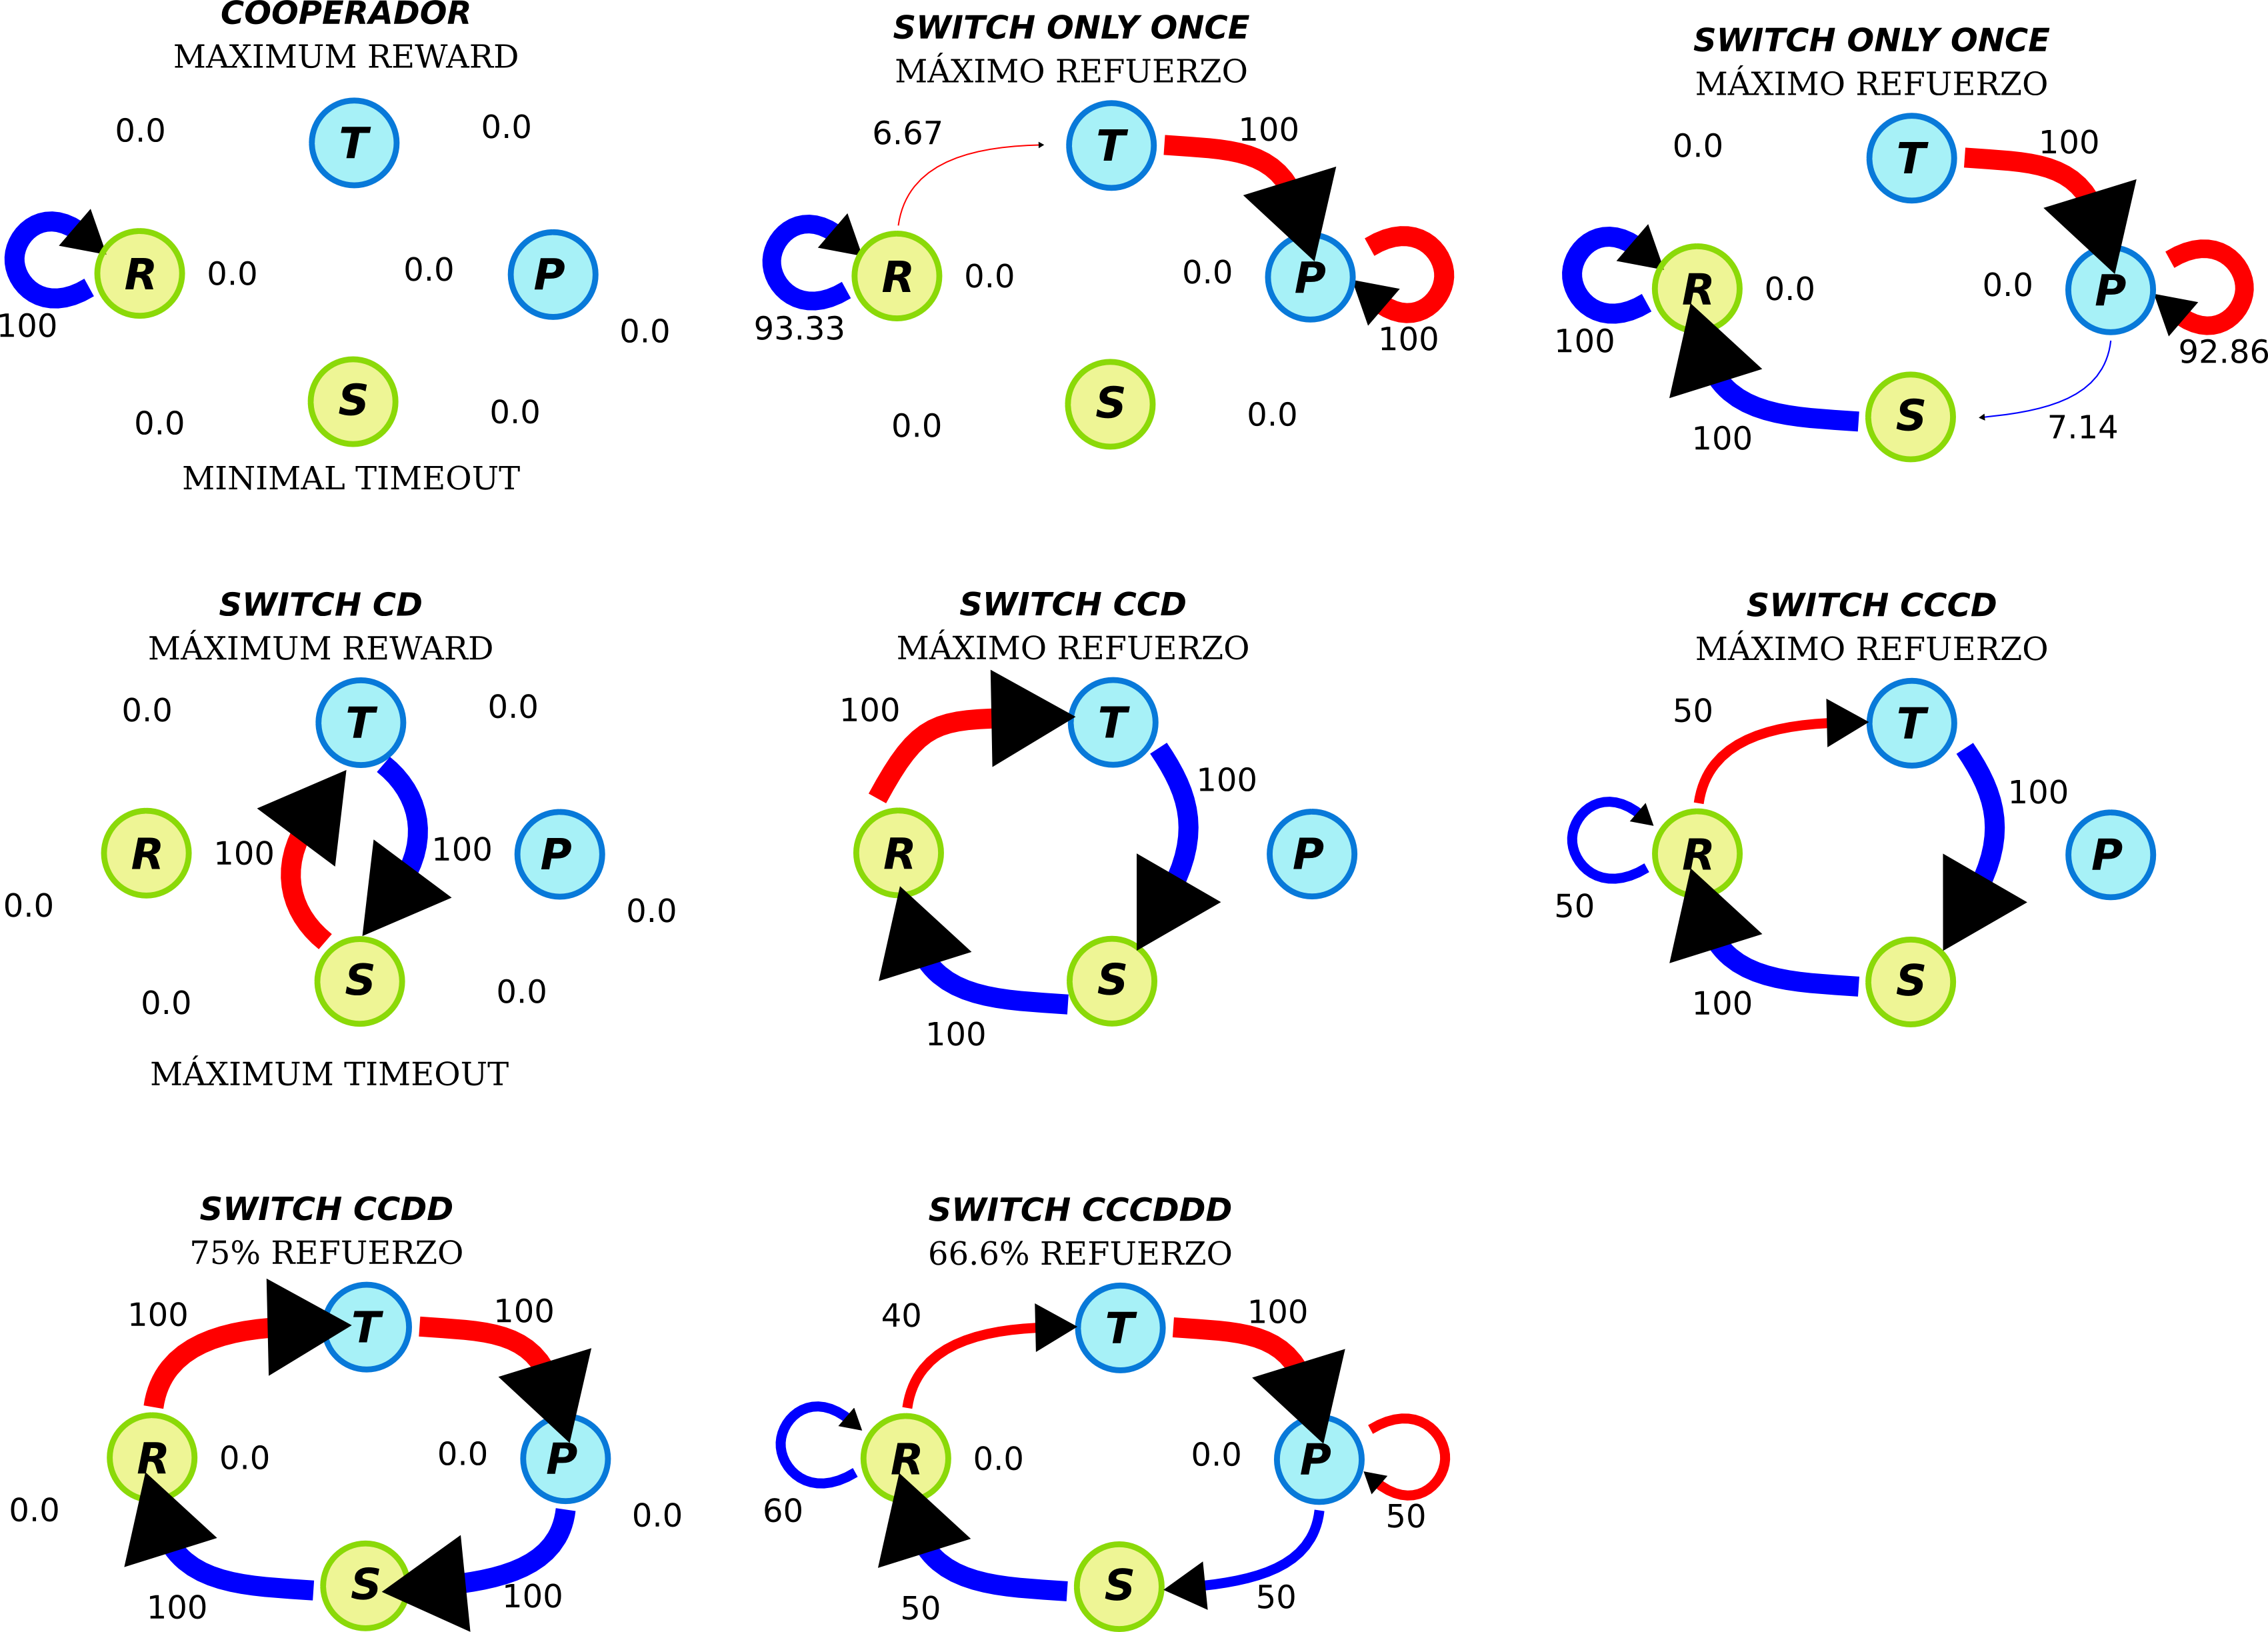
\includegraphics[width=0.95\columnwidth]{/home/guille/Documents/experimento/Experimento---iPD/ExtraerDatos/figura_iPD_1_2_9s_13s/fig_finales/Simulated_markov}

\caption{{\scriptsize{}Graph of transition probabilities.}}


\end{figure}



\subsection{Non cooperator subject Statistics}

\begin{figure}[h]
\subfloat[{\scriptsize{}Probabilities of cooperate given each outcomes}]{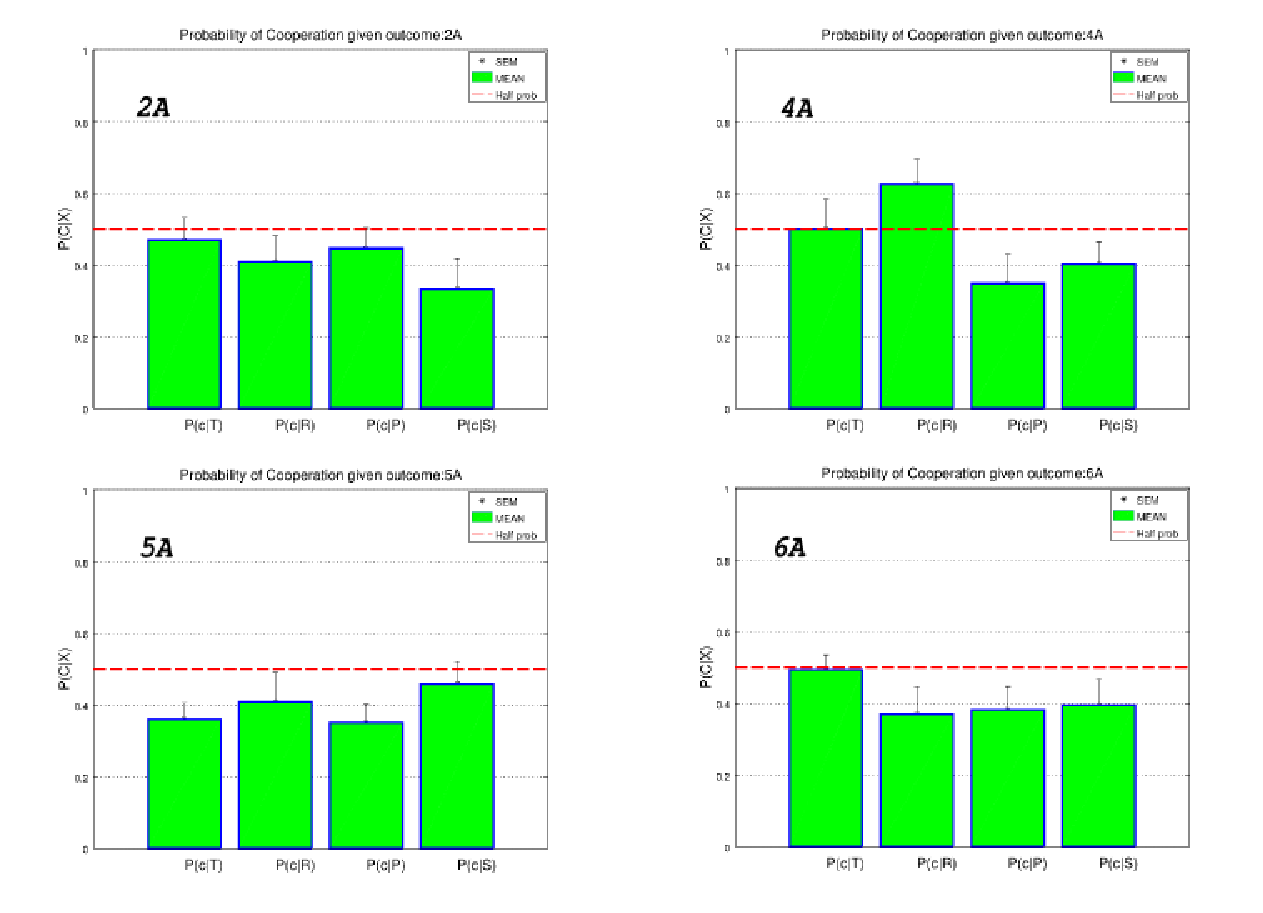
\includegraphics[width=0.95\columnwidth]{/home/guille/Documents/experimento/Experimento---iPD/ExtraerDatos/figura_iPD_1_2_9s_13s/fig_finales/nocoop_probabilidades}



\label{fig_nocoop_statistic}}

\subfloat[{\scriptsize{}Graph of markov transition probabilities per subject}]{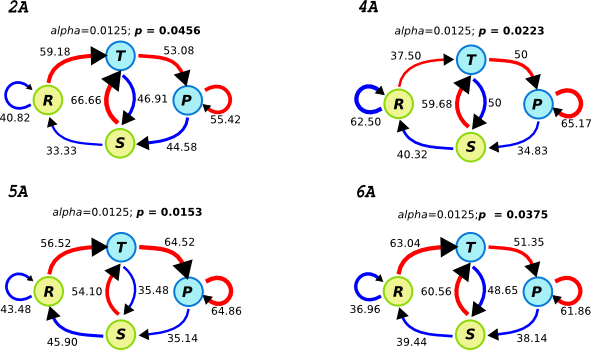
\includegraphics[width=0.95\columnwidth]{/home/guille/Documents/experimento/Experimento---iPD/ExtraerDatos/figura_iPD_1_2_9s_13s/fig_finales/nocoop_markov}



\label{fig_nocoop_markov}}

\caption{{\scriptsize{}Statistic for the removed subject. These subject had
a random behavior because. \ref{fig_nocoop_statistic}) All probabilities
of cooperate given each outcome are near 50 percent and this means
that their haven't any preference choice. See significant value of
$X^{2}$test in table \ref{table_meanAndstrategies}. \ref{fig_nocoop_markov})
The graph of markov chain show that the transition probabilities are
very closed to 50\%. }}
\end{figure}



\subsection{Cooperatos statistics}

\begin{figure}[h]
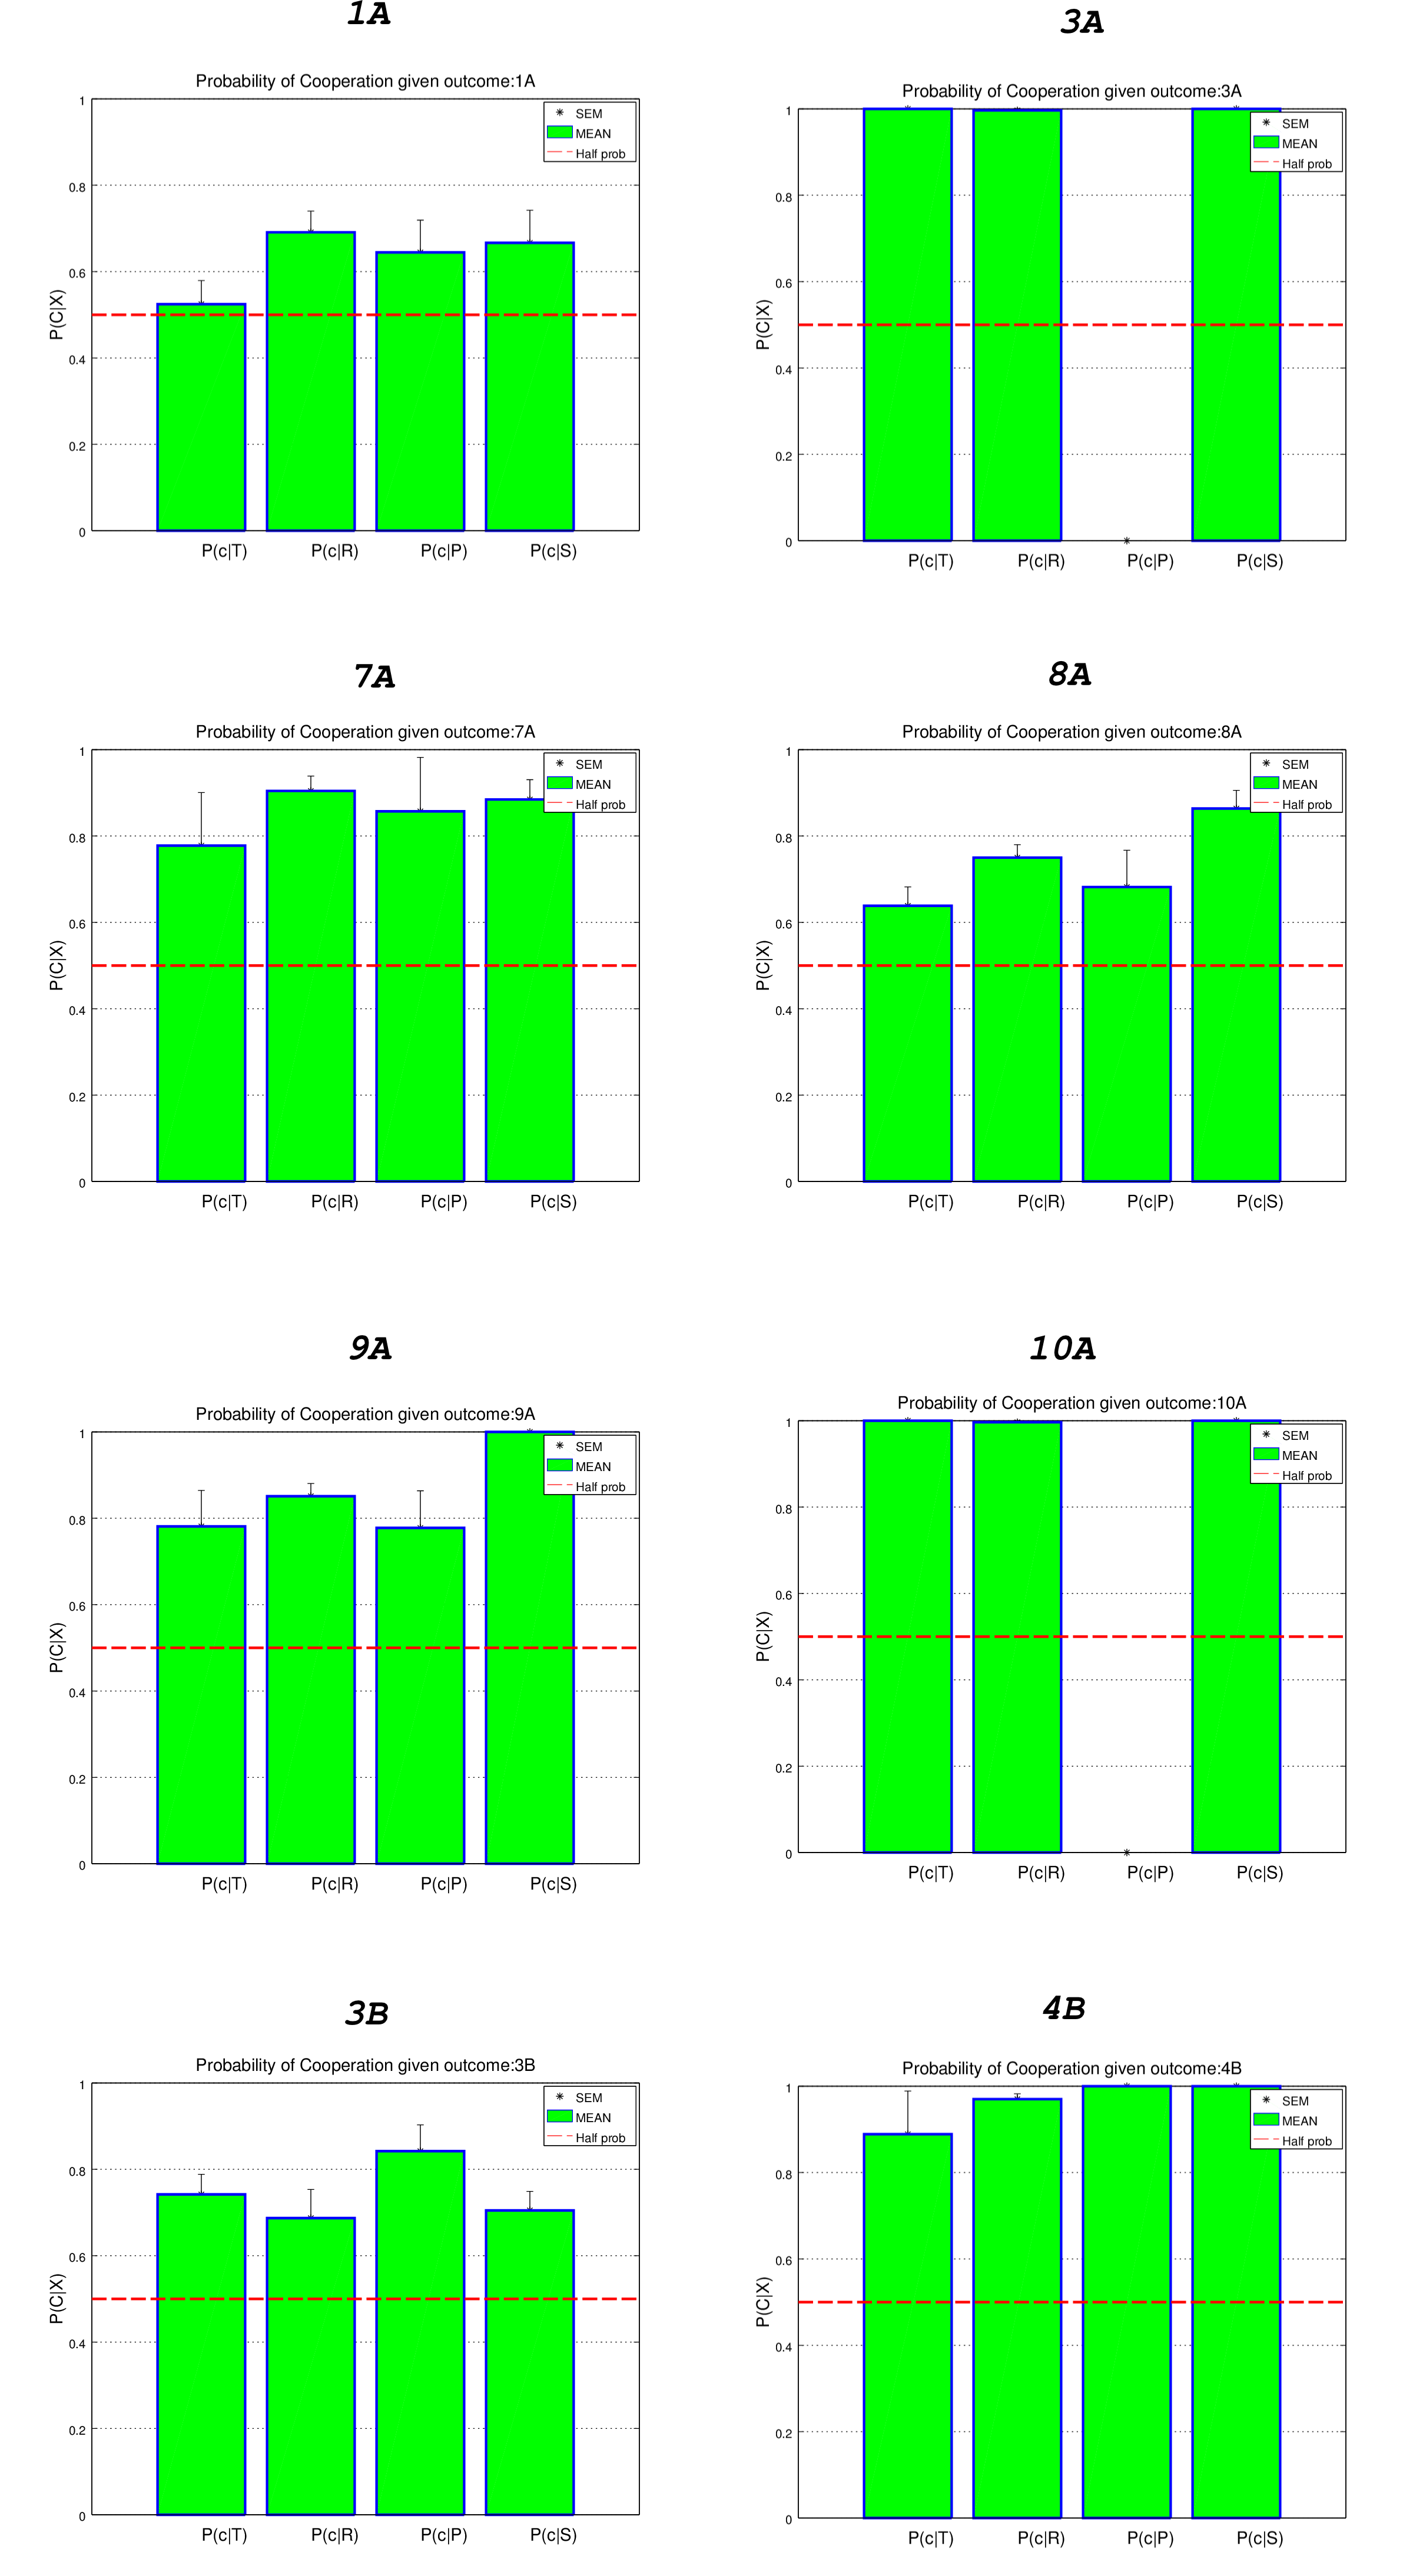
\includegraphics[width=0.9\columnwidth]{/home/guille/Documents/experimento/Experimento---iPD/ExtraerDatos/figura_iPD_1_2_9s_13s/fig_finales/coop_statistic}

\caption{Probabilities of cooperate given each outcomes for cooperator subjects
(T:temptation to cheat; R:reward when both cooperated; P:punishment's
payoff when neither cooperate;S:sucket's payoff that an altruist gets
when cheated). }


\label{fig_coop_statistic}
\end{figure}


\begin{figure}[h]
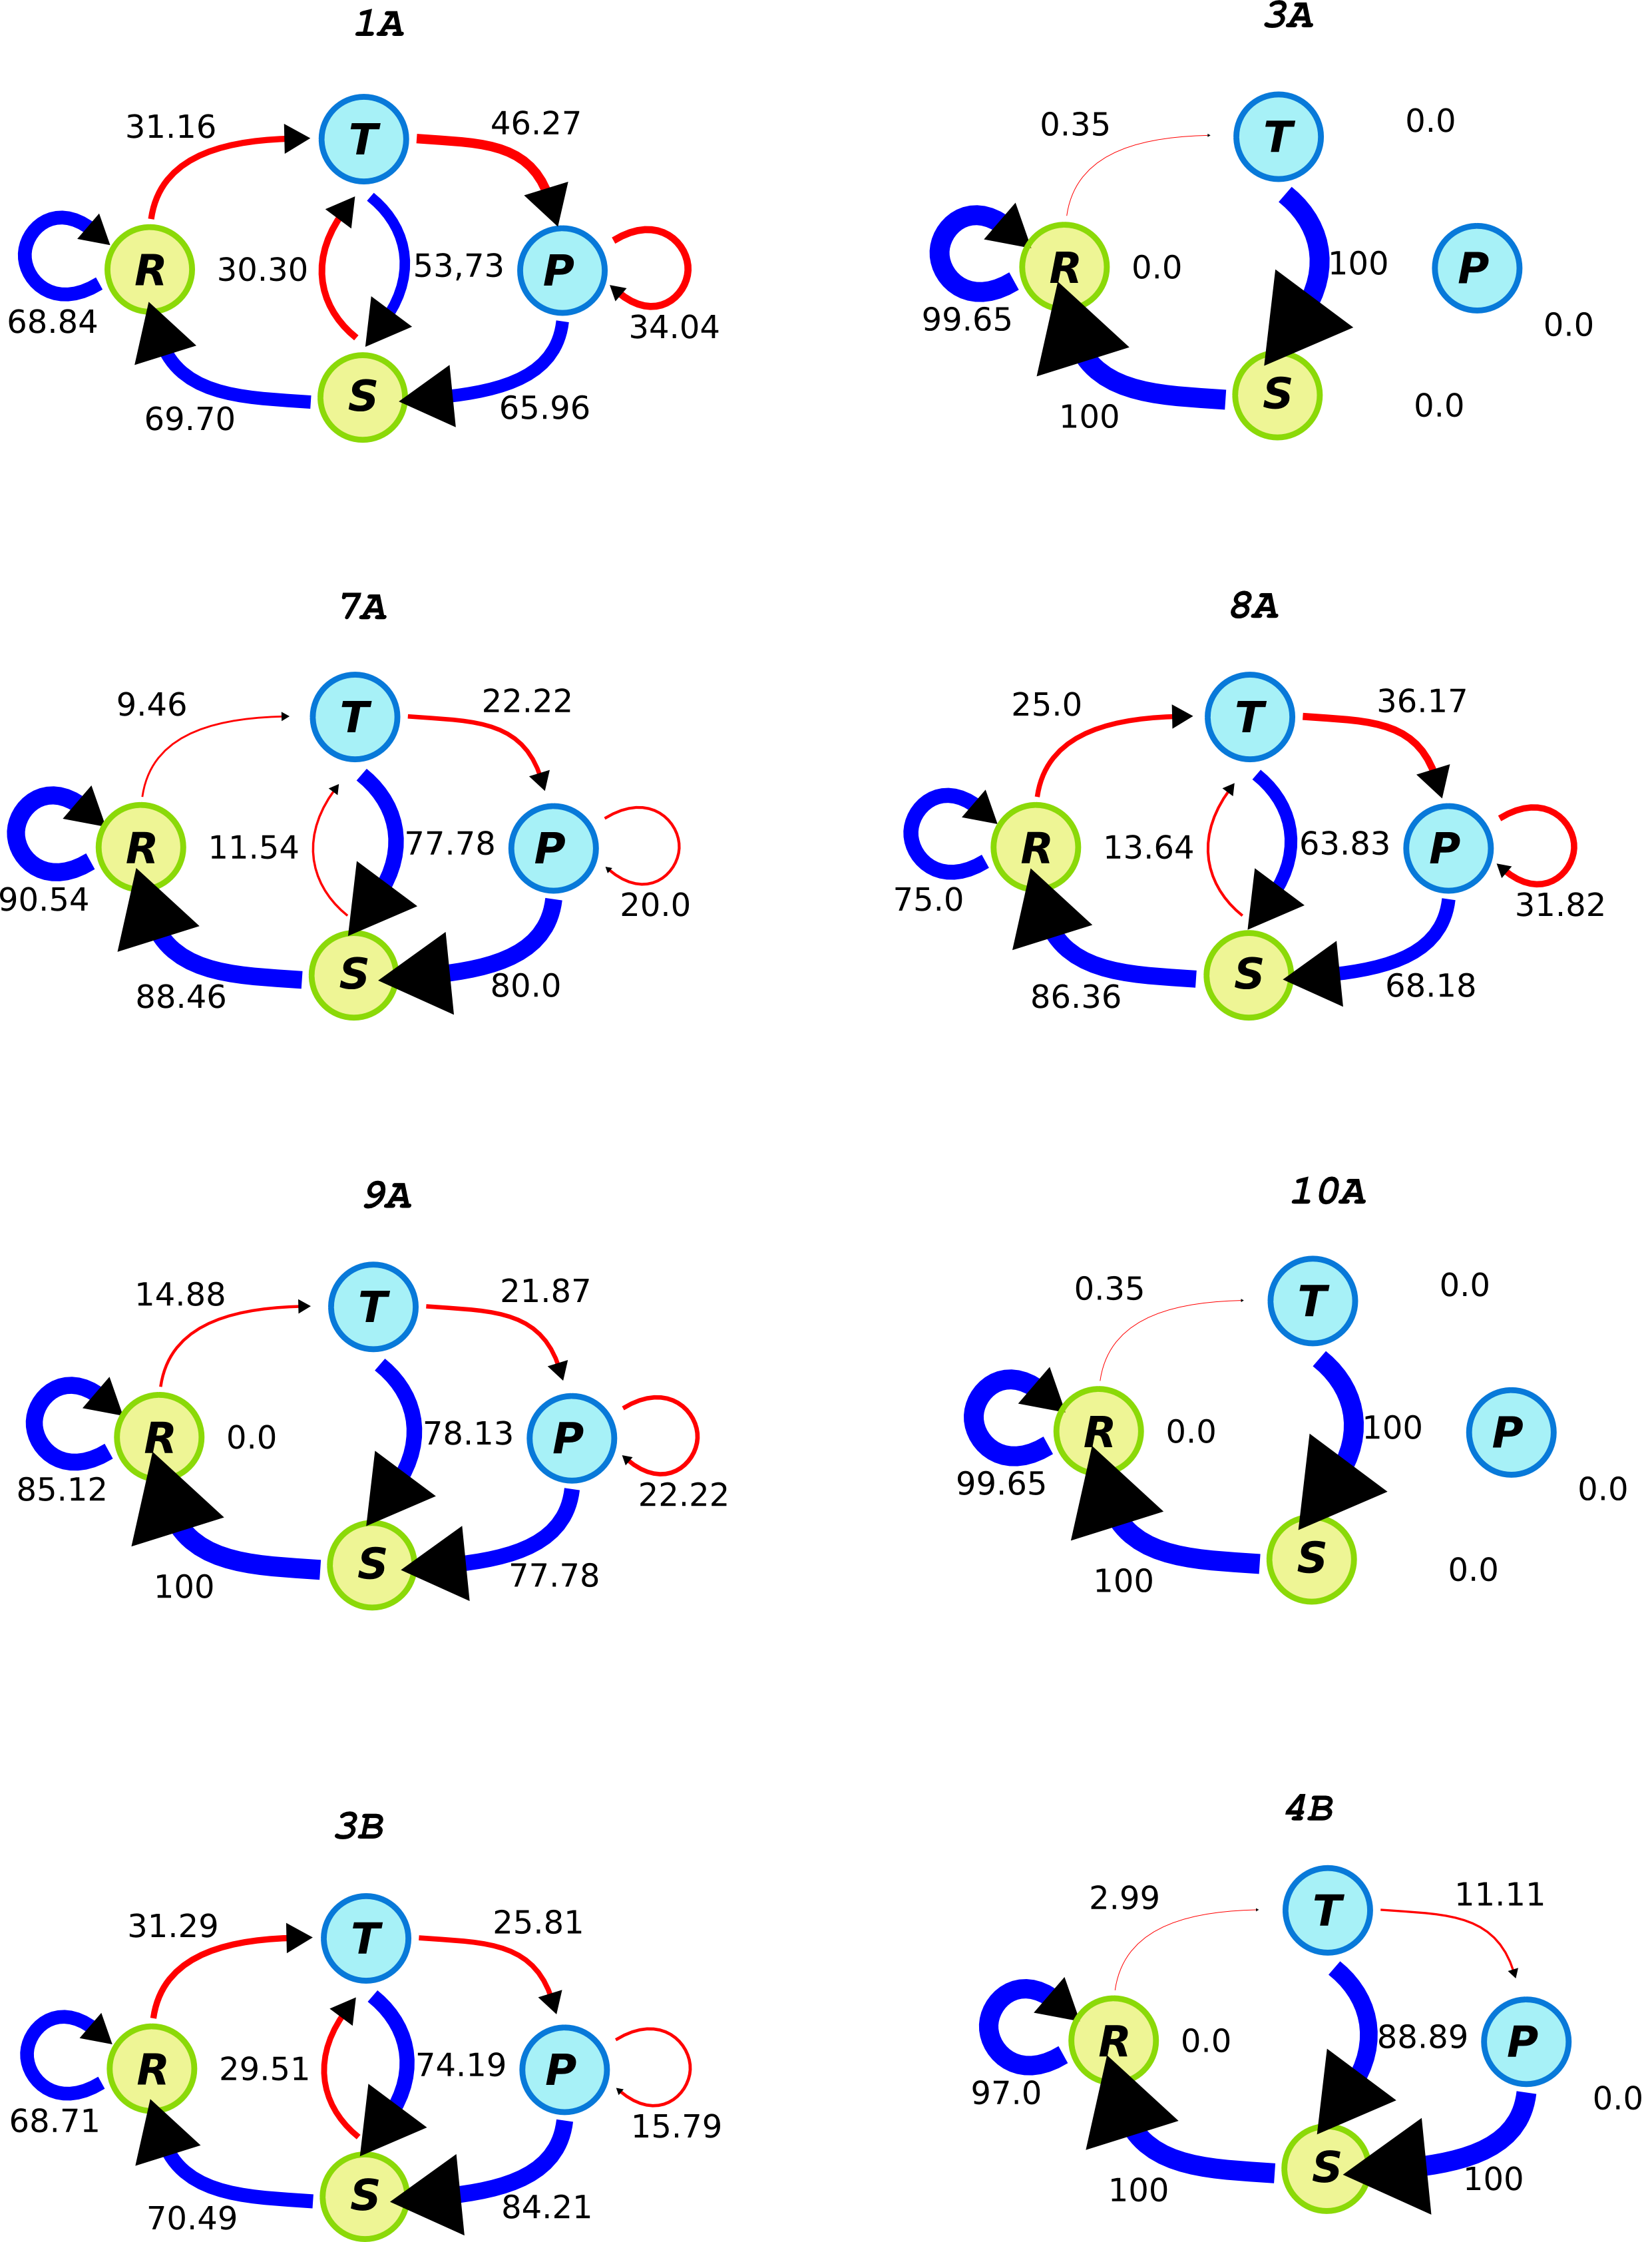
\includegraphics[width=0.95\columnwidth]{/home/guille/Documents/experimento/Experimento---iPD/ExtraerDatos/figura_iPD_1_2_9s_13s/fig_finales/coop_markov}

\caption{Graph of markov transition probabilities per subjects}


\label{fig_coop_markov}
\end{figure}

\end{document}
